\documentclass[10pt]{beamer}
% \usepackage[colorlinks=true,citecolor=blue, linkcolor=blue]{hyperref}
\usepackage{hyperref}
\usepackage[utf8x]{inputenc}
% \usepackage{algorithm, algorithmic}
% \usepackage[ruled,vlined]{algorithm2e}
% \usepackage{fontawesome}
\usepackage{graphicx}
% \usepackage[english]{babel}
\usepackage[nodayofweek]{datetime}
\usepackage{todo}
\usepackage[colorinlistoftodos]{todonotes}
\usepackage{graphicx}
\usepackage{mathtools}
\usepackage{amssymb}
\usepackage{amsmath}
\usepackage{bbm}
\usepackage{pdflscape}
\usepackage{caption}
\usepackage{subcaption}
\usepackage[T1]{fontenc}
% \usepackage[utf8]{inputenc}
\usepackage{authblk}
\usepackage{pdfpages}
\usepackage{setspace} 
\usepackage{booktabs}
\usepackage{longtable}
\usepackage{float}
\usepackage{tikz}
% \usepackage{multirow}
% \setlength{\tabcolsep}{5pt}
% \usepackage[parfill]{parskip}
% \renewcommand{\arraystretch}{1.5}

% ------------------------------------------------------------------------------
% Use the beautiful metropolis beamer template
% ------------------------------------------------------------------------------
\usepackage[T1]{fontenc}
\usepackage{fontawesome}
\usepackage{FiraSans} 
\mode<presentation>
{
  \usetheme[progressbar=foot,numbering=fraction,background=light]{metropolis} 
  \usecolortheme{default} % or try albatross, beaver, crane, ...
  \usefonttheme{default}  % or try serif, structurebold, ...
  \setbeamertemplate{navigation symbols}{}
  % \setbeamertemplate{caption}[numbered]
  %\setbeamertemplate{frame footer}{My custom footer}
} 

\setbeamertemplate{section in toc}{\hspace*{1em}\inserttocsectionnumber.~\inserttocsection\par}
\setbeamertemplate{subsection in toc}{\hspace*{2em}\inserttocsectionnumber.\inserttocsubsectionnumber.~\inserttocsubsection\par}

% ------------------------------------------------------------------------------
% beamer doesn't have texttt defined, but I usually want it anyway
% ------------------------------------------------------------------------------
\let\textttorig\texttt
\renewcommand<>{\texttt}[1]{%
  \only#2{\textttorig{#1}}%
}

% ------------------------------------------------------------------------------
% minted
% ------------------------------------------------------------------------------
\usepackage{minted}


% ------------------------------------------------------------------------------
% tcolorbox / tcblisting
% ------------------------------------------------------------------------------
\usepackage{xcolor}
\definecolor{codecolor}{HTML}{FFC300}

\usepackage{tcolorbox}
\tcbuselibrary{most,listingsutf8,minted}

\tcbset{tcbox width=auto,left=1mm,top=1mm,bottom=1mm,
right=1mm,boxsep=1mm,middle=1pt}

\newtcblisting{myr}[1]{colback=codecolor!5,colframe=codecolor!80!black,listing only, 
minted options={numbers=left, style=tcblatex,fontsize=\tiny,breaklines,autogobble,linenos,numbersep=3mm},
left=5mm,enhanced,
title=#1, fonttitle=\bfseries,
listing engine=minted,minted language=r}


% ------------------------------------------------------------------------------
% Listings
% ------------------------------------------------------------------------------
\definecolor{mygreen}{HTML}{37980D}
\definecolor{myblue}{HTML}{0D089F}
\definecolor{myred}{HTML}{98290D}

\usepackage{listings}

% the following is optional to configure custom highlighting
\lstdefinelanguage{XML}
{
  morestring=[b]",
  morecomment=[s]{<!--}{-->},
  morestring=[s]{>}{<},
  morekeywords={ref,xmlns,version,type,canonicalRef,metr,real,target}% list your attributes here
}

\lstdefinestyle{myxml}{
language=XML,
showspaces=false,
showtabs=false,
basicstyle=\ttfamily,
columns=fullflexible,
breaklines=true,
showstringspaces=false,
breakatwhitespace=true,
escapeinside={(*@}{@*)},
basicstyle=\color{mygreen}\ttfamily,%\footnotesize,
stringstyle=\color{myred},
commentstyle=\color{myblue}\upshape,
keywordstyle=\color{myblue}\bfseries,
}

% ------------------------------------------------------------------------------
% The Document
% ------------------------------------------------------------------------------

\begin{document}

\title{A clustering framework for conditional extremes models}

\date{
  \footnotesize Postgraduate Seminar Series (PSS) Talk, \\
  \today \\
  % \shortdate \\
  % \vspace{0.4cm}
  \emph{Paddy O'Toole} \\
  % \vspace{-5mm}
  \emph{Supervised by Christian Rohrbeck and Jordan Richards (University of Edinburgh)}
}

% \title{Wessex Water: Bayesian Network for Source Apportionment}
% \author{\emph{Sam Williams, Paddy O'Toole, Christian Rohrbeck, Haiyan Zheng, Emiko Dupont}}
% \date{\today}


\frame{\titlepage}

%==================================================

% \frame{\begin{small}
% \frametitle{Overview}
% \tableofcontents\end{small}}

%=================================================
\begin{frame}
\frametitle{Table of Contents}
\tableofcontents
\end{frame}

\section{Introduction}


% Images of Pulteney Bridge Weir and plaque
% Frank Greenhalgh, Engineer who designed Pulteney Weir and Sluce for Bristol Avon River Authority
\begin{frame}
   \begin{minipage}{0.49\textwidth}
     % 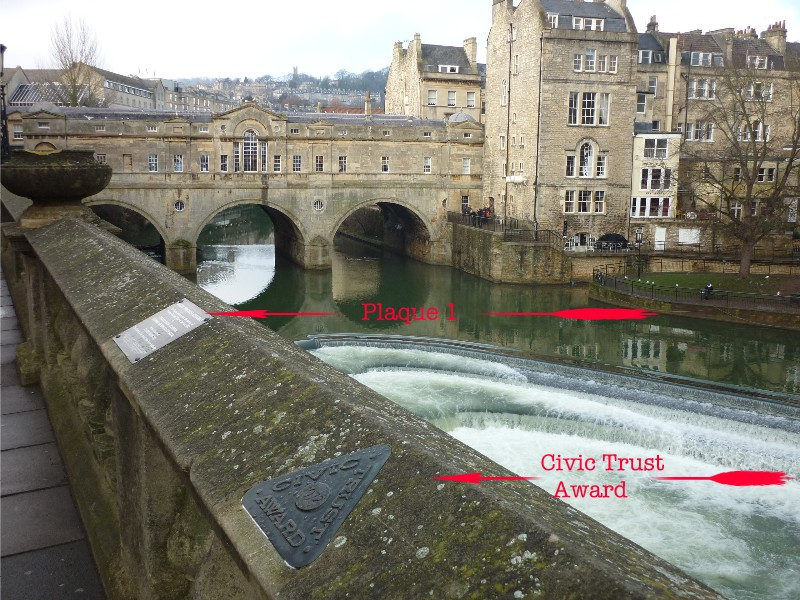
\includegraphics[width=.99\textwidth]{images/civictrustaward_location.jpg}
     \todo{Get a nicer picture of Pulteney Bridge!}
     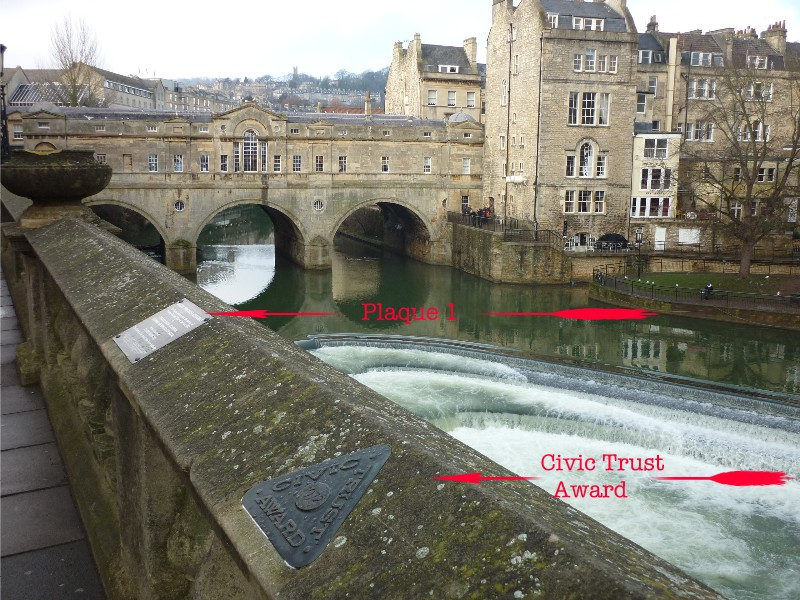
\includegraphics[width=.99\textwidth]{images/civictrustaward_location.jpg}
   \end{minipage}
   \hfill
   \begin{minipage}{0.49\textwidth}
     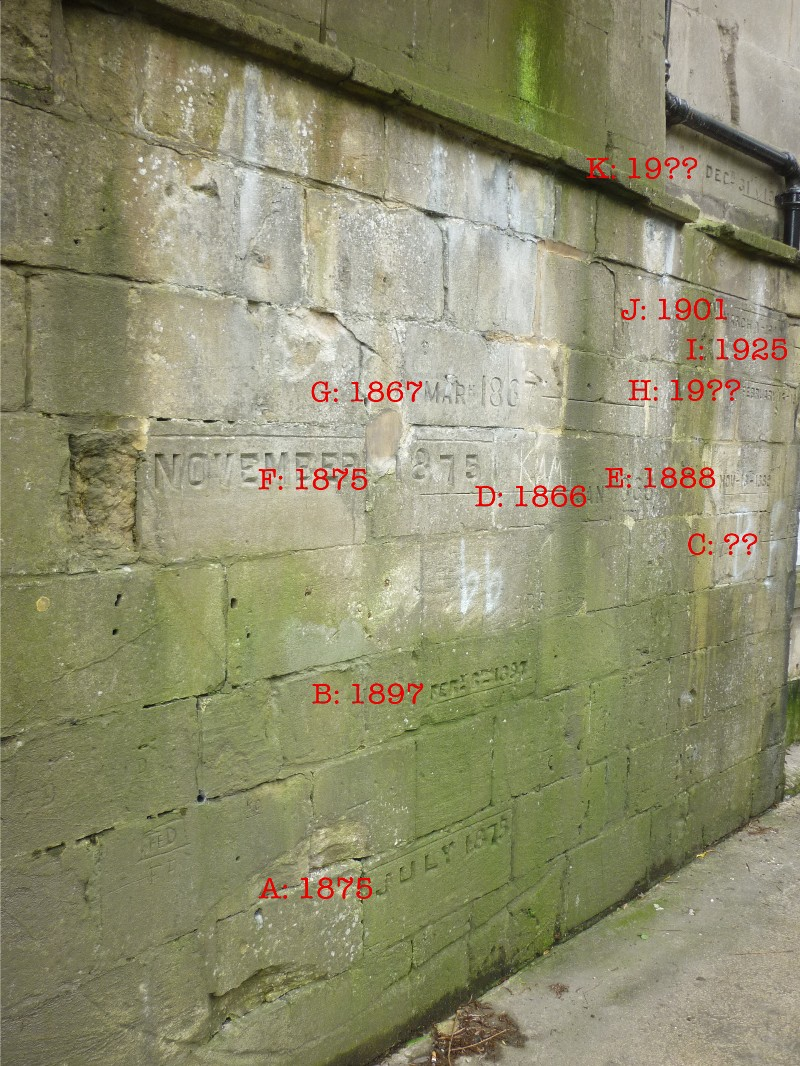
\includegraphics[width=.99\textwidth]{images/Hapennybr_lower.jpg}
   \end{minipage}
\end{frame}

% Motivation behind EVT
\begin{frame}{Introduction}
   \begin{minipage}{0.49\textwidth}
        % Anything else to add here?
        \begin{itemize}
            \item Extreme Value Theory models the extreme tails of distributions $X$. % standard models don't work well
            \item Only known method that can reliably \textbf{predict beyond observations} in extremal context.
            % \item Applications found in finance, insurance and environmental 
            \item Applications found in finance, engineering and environmental sciences.
        \end{itemize}
   \end{minipage}
   \hfill
   \begin{minipage}{0.49\textwidth}
     % \centering
     \vspace{}
     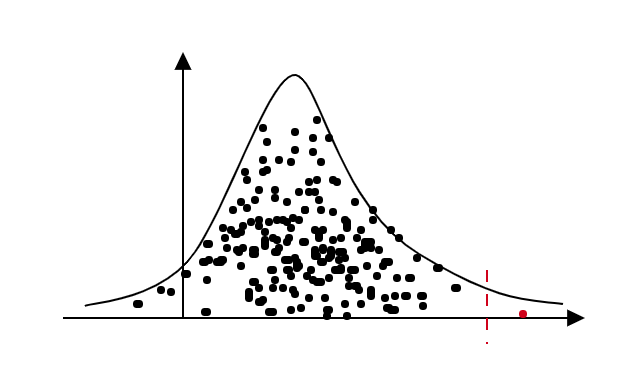
\includegraphics[width=6cm]{images/tail.png}
   \end{minipage}
\end{frame}

\begin{frame}{Problem} 
  \begin{itemize}
    \item Often we want to estimate
      \[
        \mathbb{P}(X > x, Y > y) = \textcolor{red}{\mathbb{P}(Y > y \mid X > x)}\textcolor{blue}{\mathbb{P}(X > x)}
      \]
      for large $x, y$.
    \todo{Remove as bullets and just say outloud?}
    \item $X, Y$ could represent meterological data for a single location, or a single variable at multiple locations. 
    \item This probability may represent a particularly destructive event, like a storm, where we may observe ``concomitant'' extremes of precipitation and wind speed.
    \item The \textcolor{blue}{second term} can be modelled using a marginal model such as the \textbf{Generalised Pareto distribution} (GPD).
    \item The \textcolor{red}{first term} involves modelling the \textbf{dependence} between $X$ and $Y$, which is more difficult.
  \end{itemize}
\end{frame}

% \begin{frame}{Generalised Pareto Distribution}
%   \todo{How/where to situate this within presentation?}
% The GPD is often characterised by it's survival function:
% \begin{equation*} 
%   \mathbb{P}(X > x + u \mid X > u) = \left(1 + \xi \frac{x}{\sigma} \right)_{+}^{-1/\xi},
% \end{equation*}
% \vspace{-5mm}
% \begin{itemize}
%     \item $(x)_+ = \max{(0, x)}$
%     \item Parameters: scale $\sigma$, shape $\xi$, 
%     % \item For $\xi < 0$, (increasingly small) finite upper end point
%     % \item Can model parameters as function of spatial location, i.e.\ $\sigma(s), \xi(s)$, with $s =$ (longitude, latitude)
%     \item Threshold $u$ often taken as high quantile of data. % , can also model as $u(s)$
% \end{itemize}
% \end{frame}

% % MV extremes, uses, methods, shortcomings - clustering
% % todo: Add 2D plot showing different regions of extremity
% \begin{frame}{Multivariate extremes}
%     \begin{itemize}
%       \item Concurrently occurring extremal events can be particularly destructive 
%       \item $\mathbb{P}(\bm{X} \in \bm{C}) = \sum_{i=1}^{d}{\mathbb{P}(\bm{X}_i \in C_i)}$, for some extreme set $C_i$ corresponding to each vector $X_i$. 
%       \item This may refer to different spatial locations, or different variables
%       \item For example, offshore platforms must be built to withstand extreme wind speed and wave height conditions at sea
%       \item Storm defences must withstand extreme rainfall and wind speed conditions, and insurance premiums must take into account these particularly destructive events
%     \end{itemize}
% \end{frame}
% 
% \begin{frame}{Multivariate extremes}
%      % 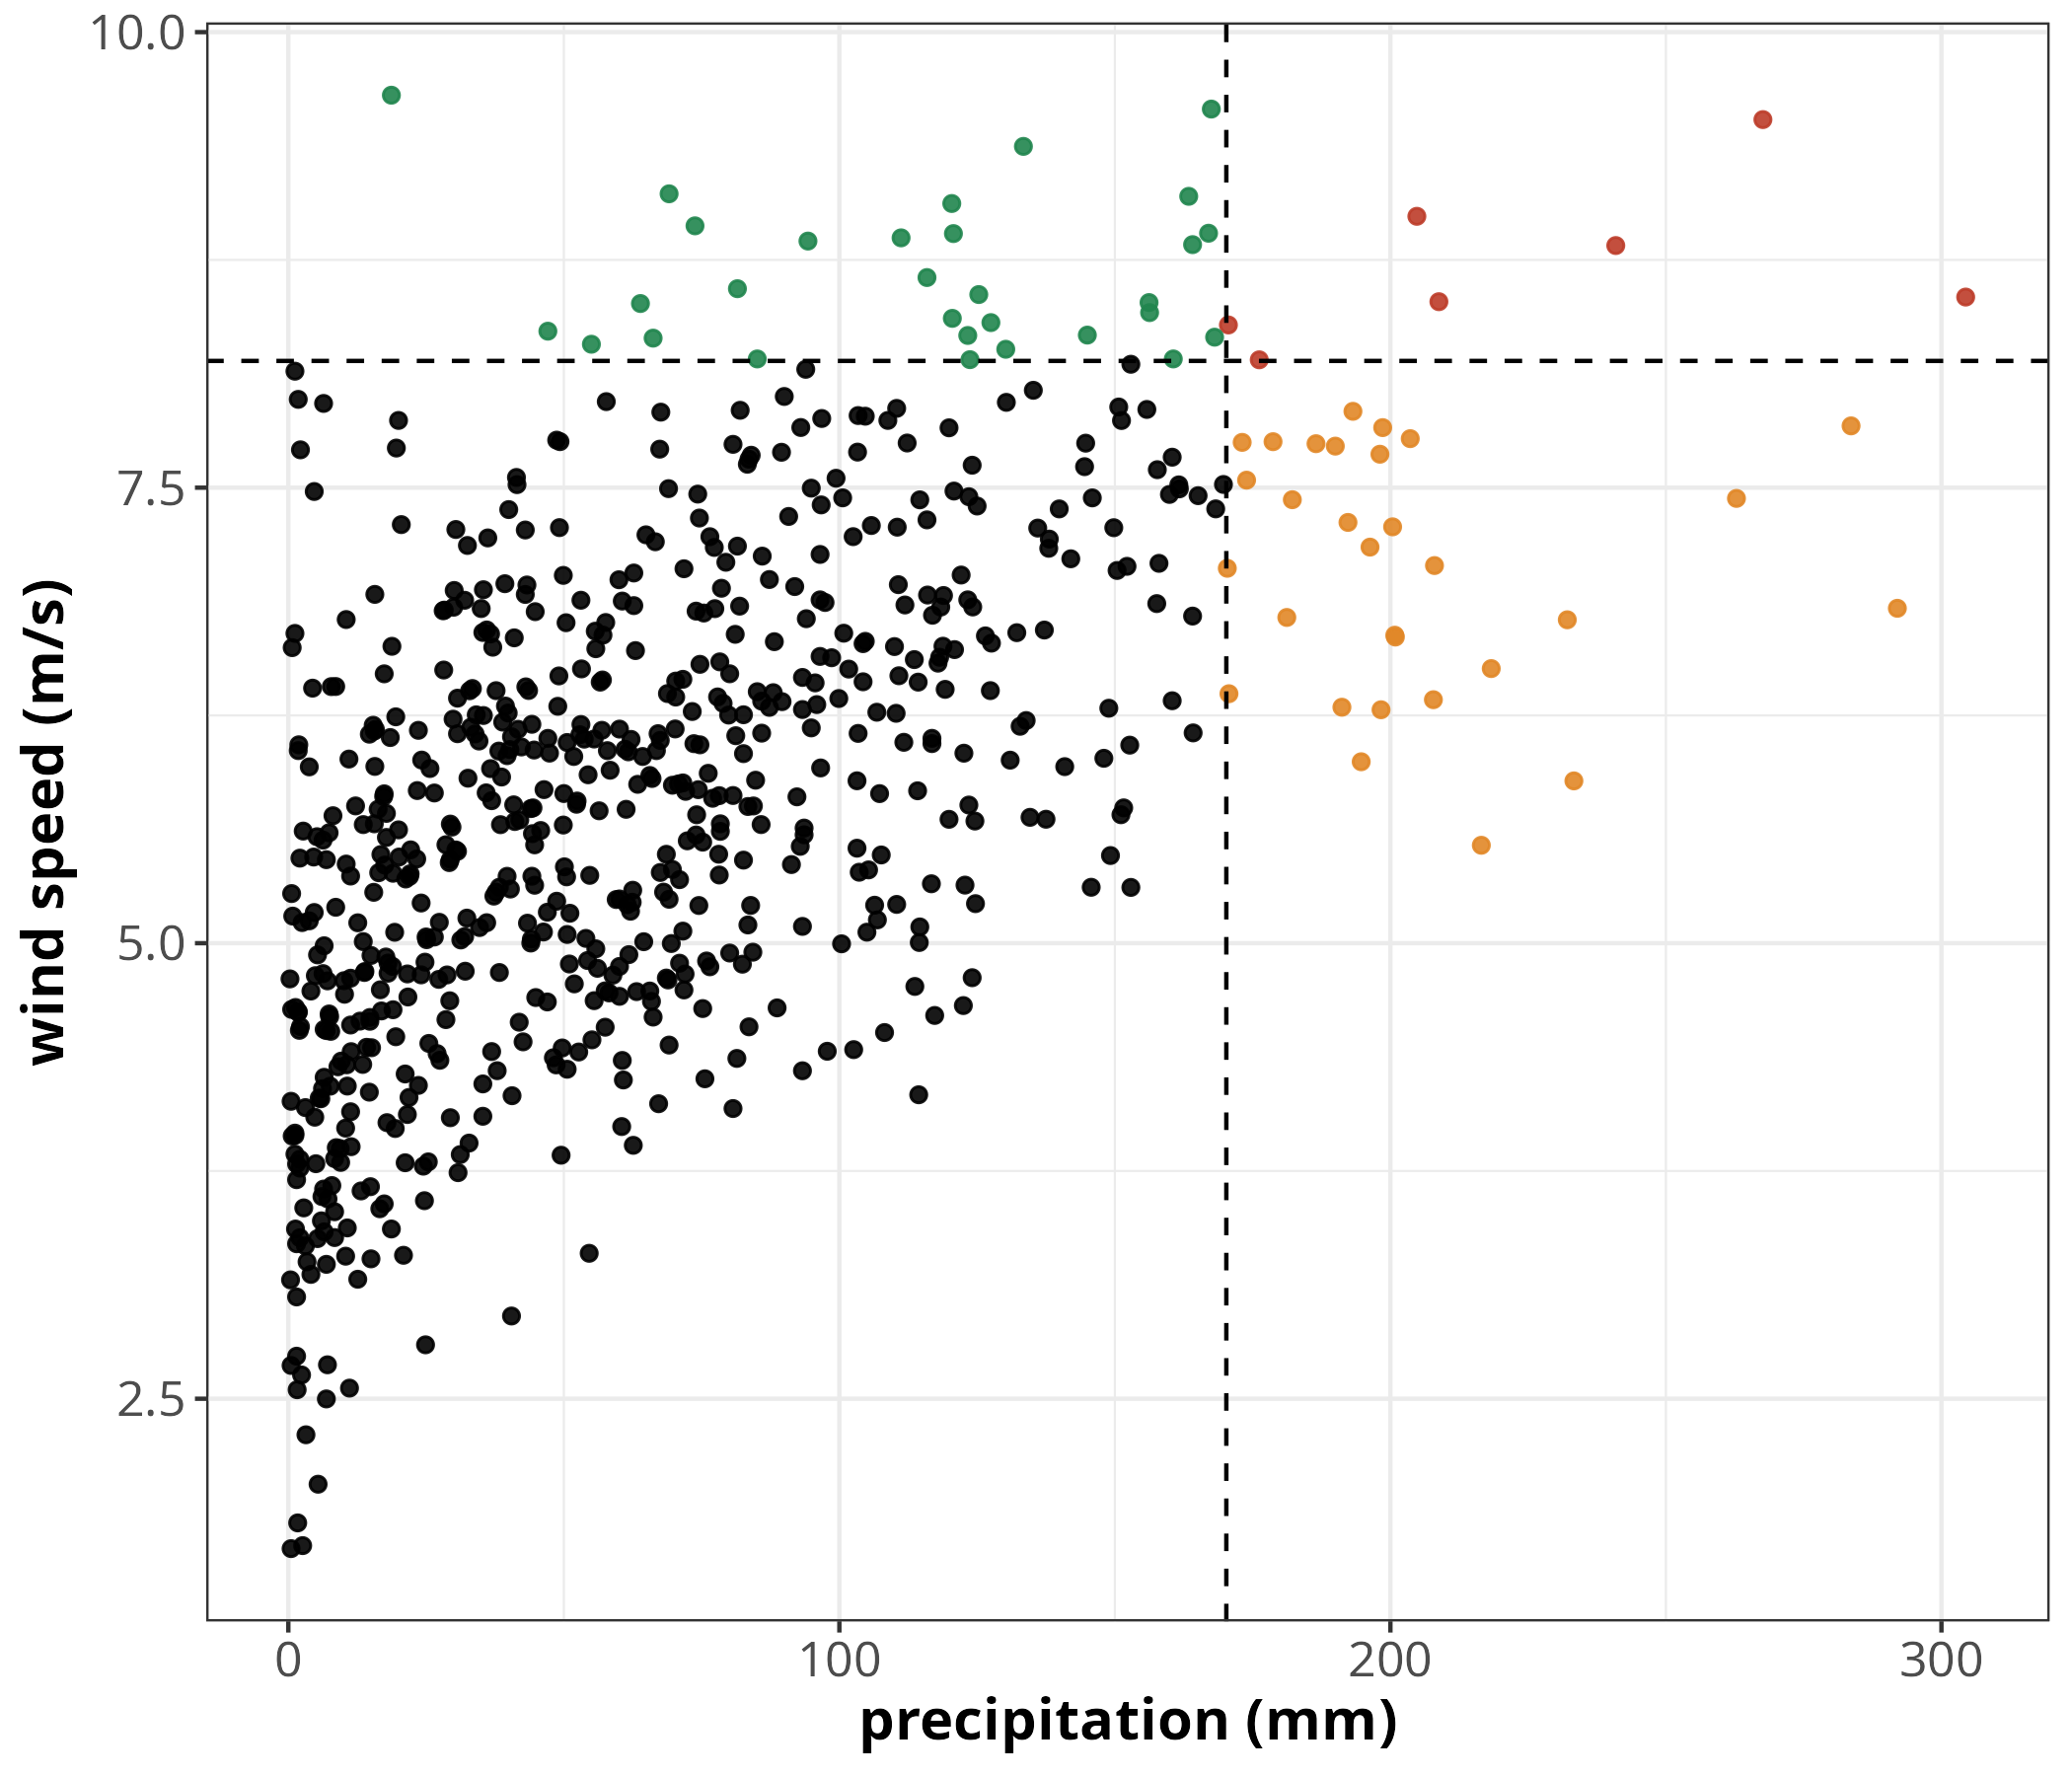
\includegraphics[width=.9\textwidth]{plots/021_mv_extreme.png}
% \end{frame}

\begin{frame}{Aims}
  \begin{enumerate}
    \item Give a general introduction to (asymptotic) dependence,
    \item Explain our choice of extremal dependence model, the \textbf{conditional extremes} (CE) model,
    \item Motivate and describe the clustering algorithm we propose for CE,
    \item Use simulation study and Irish meteorological application that this clustering can be used successfully to improve CE interpretability.
  \end{enumerate}

\end{frame}

\section{Dependence Modelling}

\begin{frame}{Asymptotic Dependence}
\begin{itemize}
  \item Asymptotic dependence is a measure of the strength of dependence between two random variables in the tail of their distribution.
  \item Can occur even in the absence of ``bulk'' dependence.
  \item The coefficient of dependence, $\chi \in [0, 1]$, measures the degree of extremal dependence between $X$ and $Y$ with corresponding CDFs $F_1$ and $F_2$.
  \item Defined as $\chi = \lim_{u \rightarrow 1}{\chi(u)}$, where
\[
\chi(u) = 2 - \frac{\log\left(\mathbb{P}(F_1(X) < u, F_2(Y) < u)\right)}{\log \left(\mathbb{P}(F_1(X) < u)\right)}. % log ratio of joint to marginal CDF as threshold increases
\]
\end{itemize}
\end{frame}

\begin{frame}{Asymptotic Dependence}
\begin{minipage}{0.4\textwidth}
    \begin{itemize}
      % \item $\chi$ gives limit probability of extreme $X$ given $Y$ is extreme.
      % $\item We expect joint probability of concomitant extremal events to be greater where $\chi$ is higher. % \citep{Rohrbeck2021}.
      \item If $\chi = 0$, $X, Y$ are asymptotically independent, while for $\chi > 0$, we see (increasingly strong) asymptotic dependence.
      % \item But, $\chi$ is just a summary statistic, and cannot be used to perform further inference; for this, we need a dependence model.
      \item But $\chi$ is only a summary; a \textbf{model} for dependence is needed for further inference. 
    \end{itemize}
\end{minipage}
\hfill
\begin{minipage}{0.59\textwidth}
     \vspace{}
     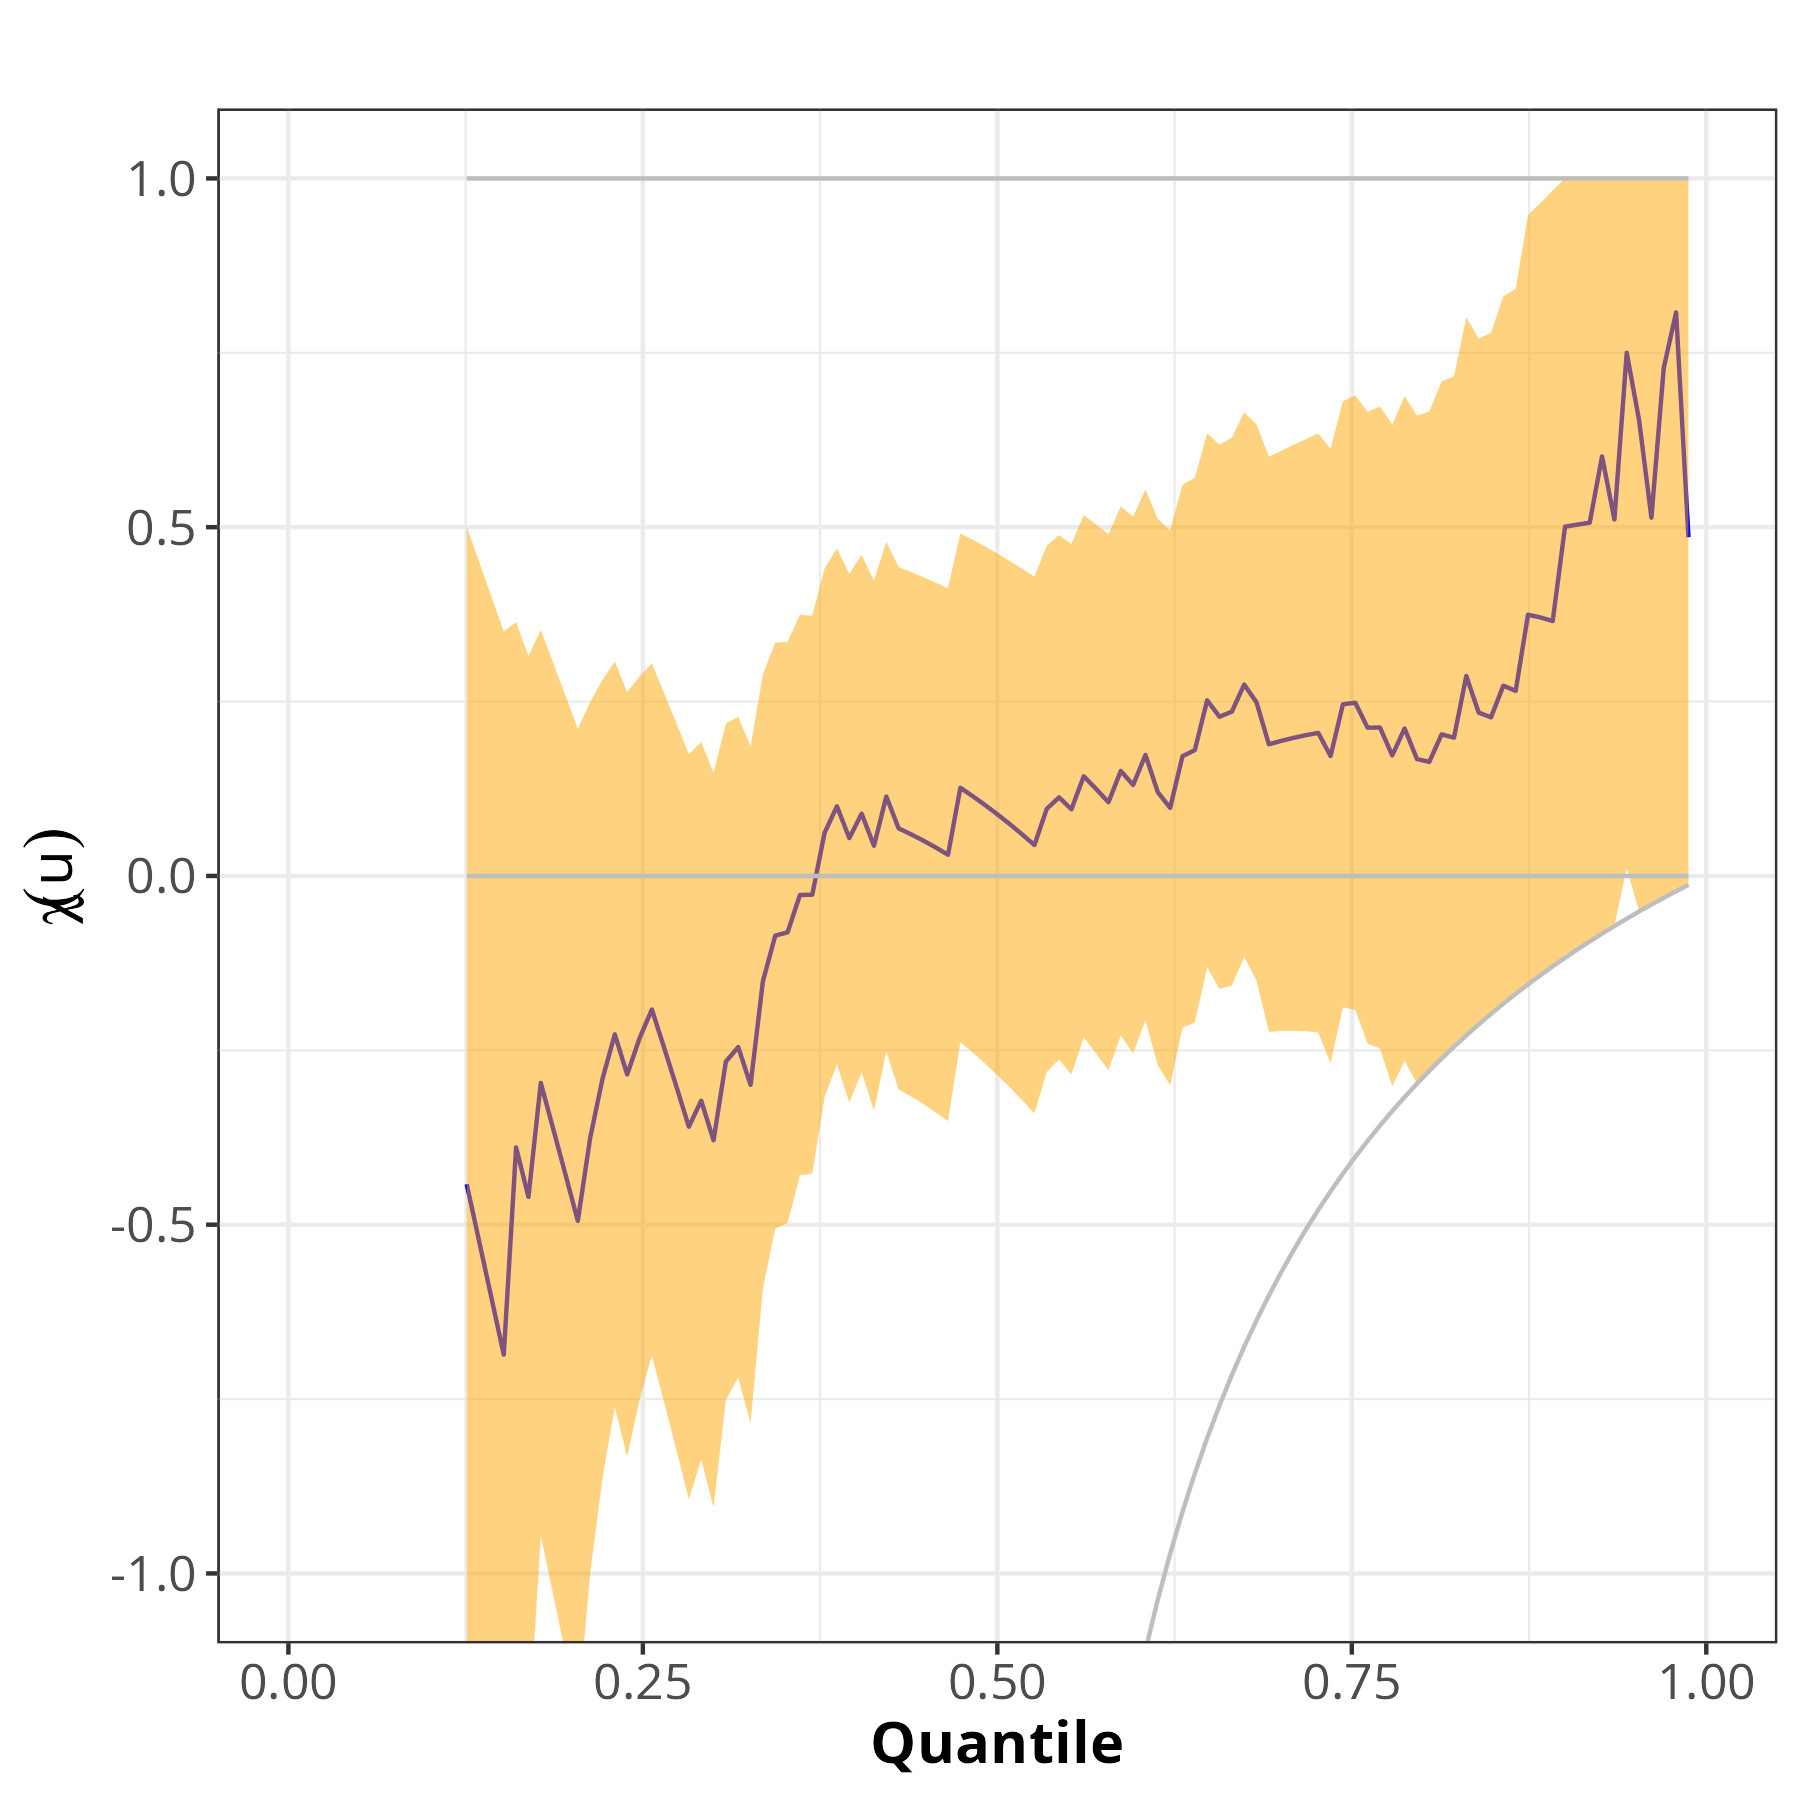
\includegraphics[width=7cm]{plots/p_chi.png}
\end{minipage}
\end{frame}

\begin{frame}{Copulas}
  \begin{itemize}
    \item One form of dependence model is a \textbf{copula}.
    \item Takes the form of a multivariate CDF with Uniform $[0, 1]$ margins:
      \begin{align*}
        C(u_1,\dots,u_d) &= F\bigl(F_1^{-1}(u_1),\dots,F_d^{-1}(u_d)\bigr) \\
                         % &= \mathbb{P}(F_1(X_1) < u_1, \dots, F_d(X_d) < u_d)
      \end{align*}
    \item \vspace{-8mm} Models marginals and joint dependence separately, margins can be any distribution.
    \item Some choices include:
      \begin{itemize}
        \item Gaussian: 
          \[
            C_{\Sigma}(u) = \Phi_{\Sigma}\Bigl(\Phi^{-1}(u_1),\dots,\Phi^{-1}(u_d)\Bigr)
          \]
        \item Student-t:
          \[
            C_{\Sigma,\nu}(u) = t_{\Sigma,\nu}\Bigl(t_\nu^{-1}(u_1),\dots,t_\nu^{-1}(u_d)\Bigr)
          \]
      \end{itemize}
    \item Often lack the flexibility of CE for modelling dependence, but \textbf{can be used to easily simulate data}.
    % Other disadvantages: Assume same dependence strength across all quantiles,
    % computationally challenging for higher dimensions, lack flexibility,
    % being fully parametric
  \end{itemize}
\end{frame}

\section{Conditional extremes}
% \begin{frame}{Introduction}
% \begin{itemize}
%   \item Gets name from modelling \emph{conditional} on a single variable, i.e. $\bm{X}_{-i} \mid X_i$ for a random vector $\bm{X}$.
%     \item Has simple univariate and dependence components
%     \item Flexible model which can model all forms of extremal dependence, such as:
%       \begin{itemize}
%         \item Asymptotic independence $(P(X_i > x_i \mid X_j > x_j) = P(X_i > x_i)$, for large $x$. 
%         \item Perfect dependence, where $X_i$ only extreme when $Y_j$ is also extreme.
%         \item Anywhere in between!
%       \end{itemize}
%     % \item Some definitions:
%     % \begin{itemize}
%     %     \item $\bm{X}_{-i}$: Vector $\bm{X}$ without $i^{th}$ component
%     %     \item $\bm{\alpha}_{\mid i}$: Vector of parameters $\alpha_{j \mid i}$ conditional on $X_i$, $j \ne i$
%     % \end{itemize}
% \end{itemize}
% \end{frame}

% semi-parametric piecewise function of empirical distribution below threshold and GPD (from previous section) above threshold:

% Univariate piecewise function
% \begin{frame}{Univariate}
%   \todo{Include a plot here?}
%   \begin{itemize}
%     \item Univariate component of model: 
%     \begin{equation*} 
%       \hat{F}_{X_i}(x) = \begin{cases}
%         1 - \{ 1 - \tilde{F}_{X_i}(u_{X_i})\} \left\{1 + \xi_{i}(x - u_{X_i})/\sigma_i\right\}_{+}^{-1/\xi_{i}} & \text{if } x > u_{X_i} \\
%         \tilde{F}_{X_i}(x) & \text{if } x \le u_{X_i},
%       \end{cases}
%     \end{equation*}
%     where $\tilde{F}_{X_i}$ is the empirical distribution function of $X_i$.
%     \item semi-parametric piecewise function of ECDF below threshold and GPD above threshold.
% \end{itemize}
% \end{frame}

% Transform to Laplace
\begin{frame}{Marginal transformation}
  \todo{Include plot of data before and after marginal transformation}
  \begin{itemize}
  \item In extremes, models often involve a transformation to more favourable margins.
  \item First, we take the piecewise CDF $F(X_i)$ with GPD above threshold and ECDF below.
  \item For CE, we transform to Laplace margins:
  \begin{equation*}
    Y_i = \begin{cases}
      % \exp(y)/2 &\text{ for } y < 0 \\
      \log\left\{2F_{X_i}(X_i)\right\} &\text{ for } X_i < F_{X_i}^{-1}(0.5), \\
      -\log\left\{2(1 - F_{X_i}(X_i))\right\} &\text{ for } X_i \ge F_{X_i}^{-1}(0.5), \\
    \end{cases}
  \end{equation*}
  \vspace{-5mm}
  \item Both tails exponential with mean 1, which is more convenient to model. 
  \end{itemize}
\end{frame}

\begin{frame}{Marginal transformation}
% allows for heteroskedastic regression model, symmetry means model is the same
  % for both positive and negative dependence, and also easy to model any
  % dependence strength
  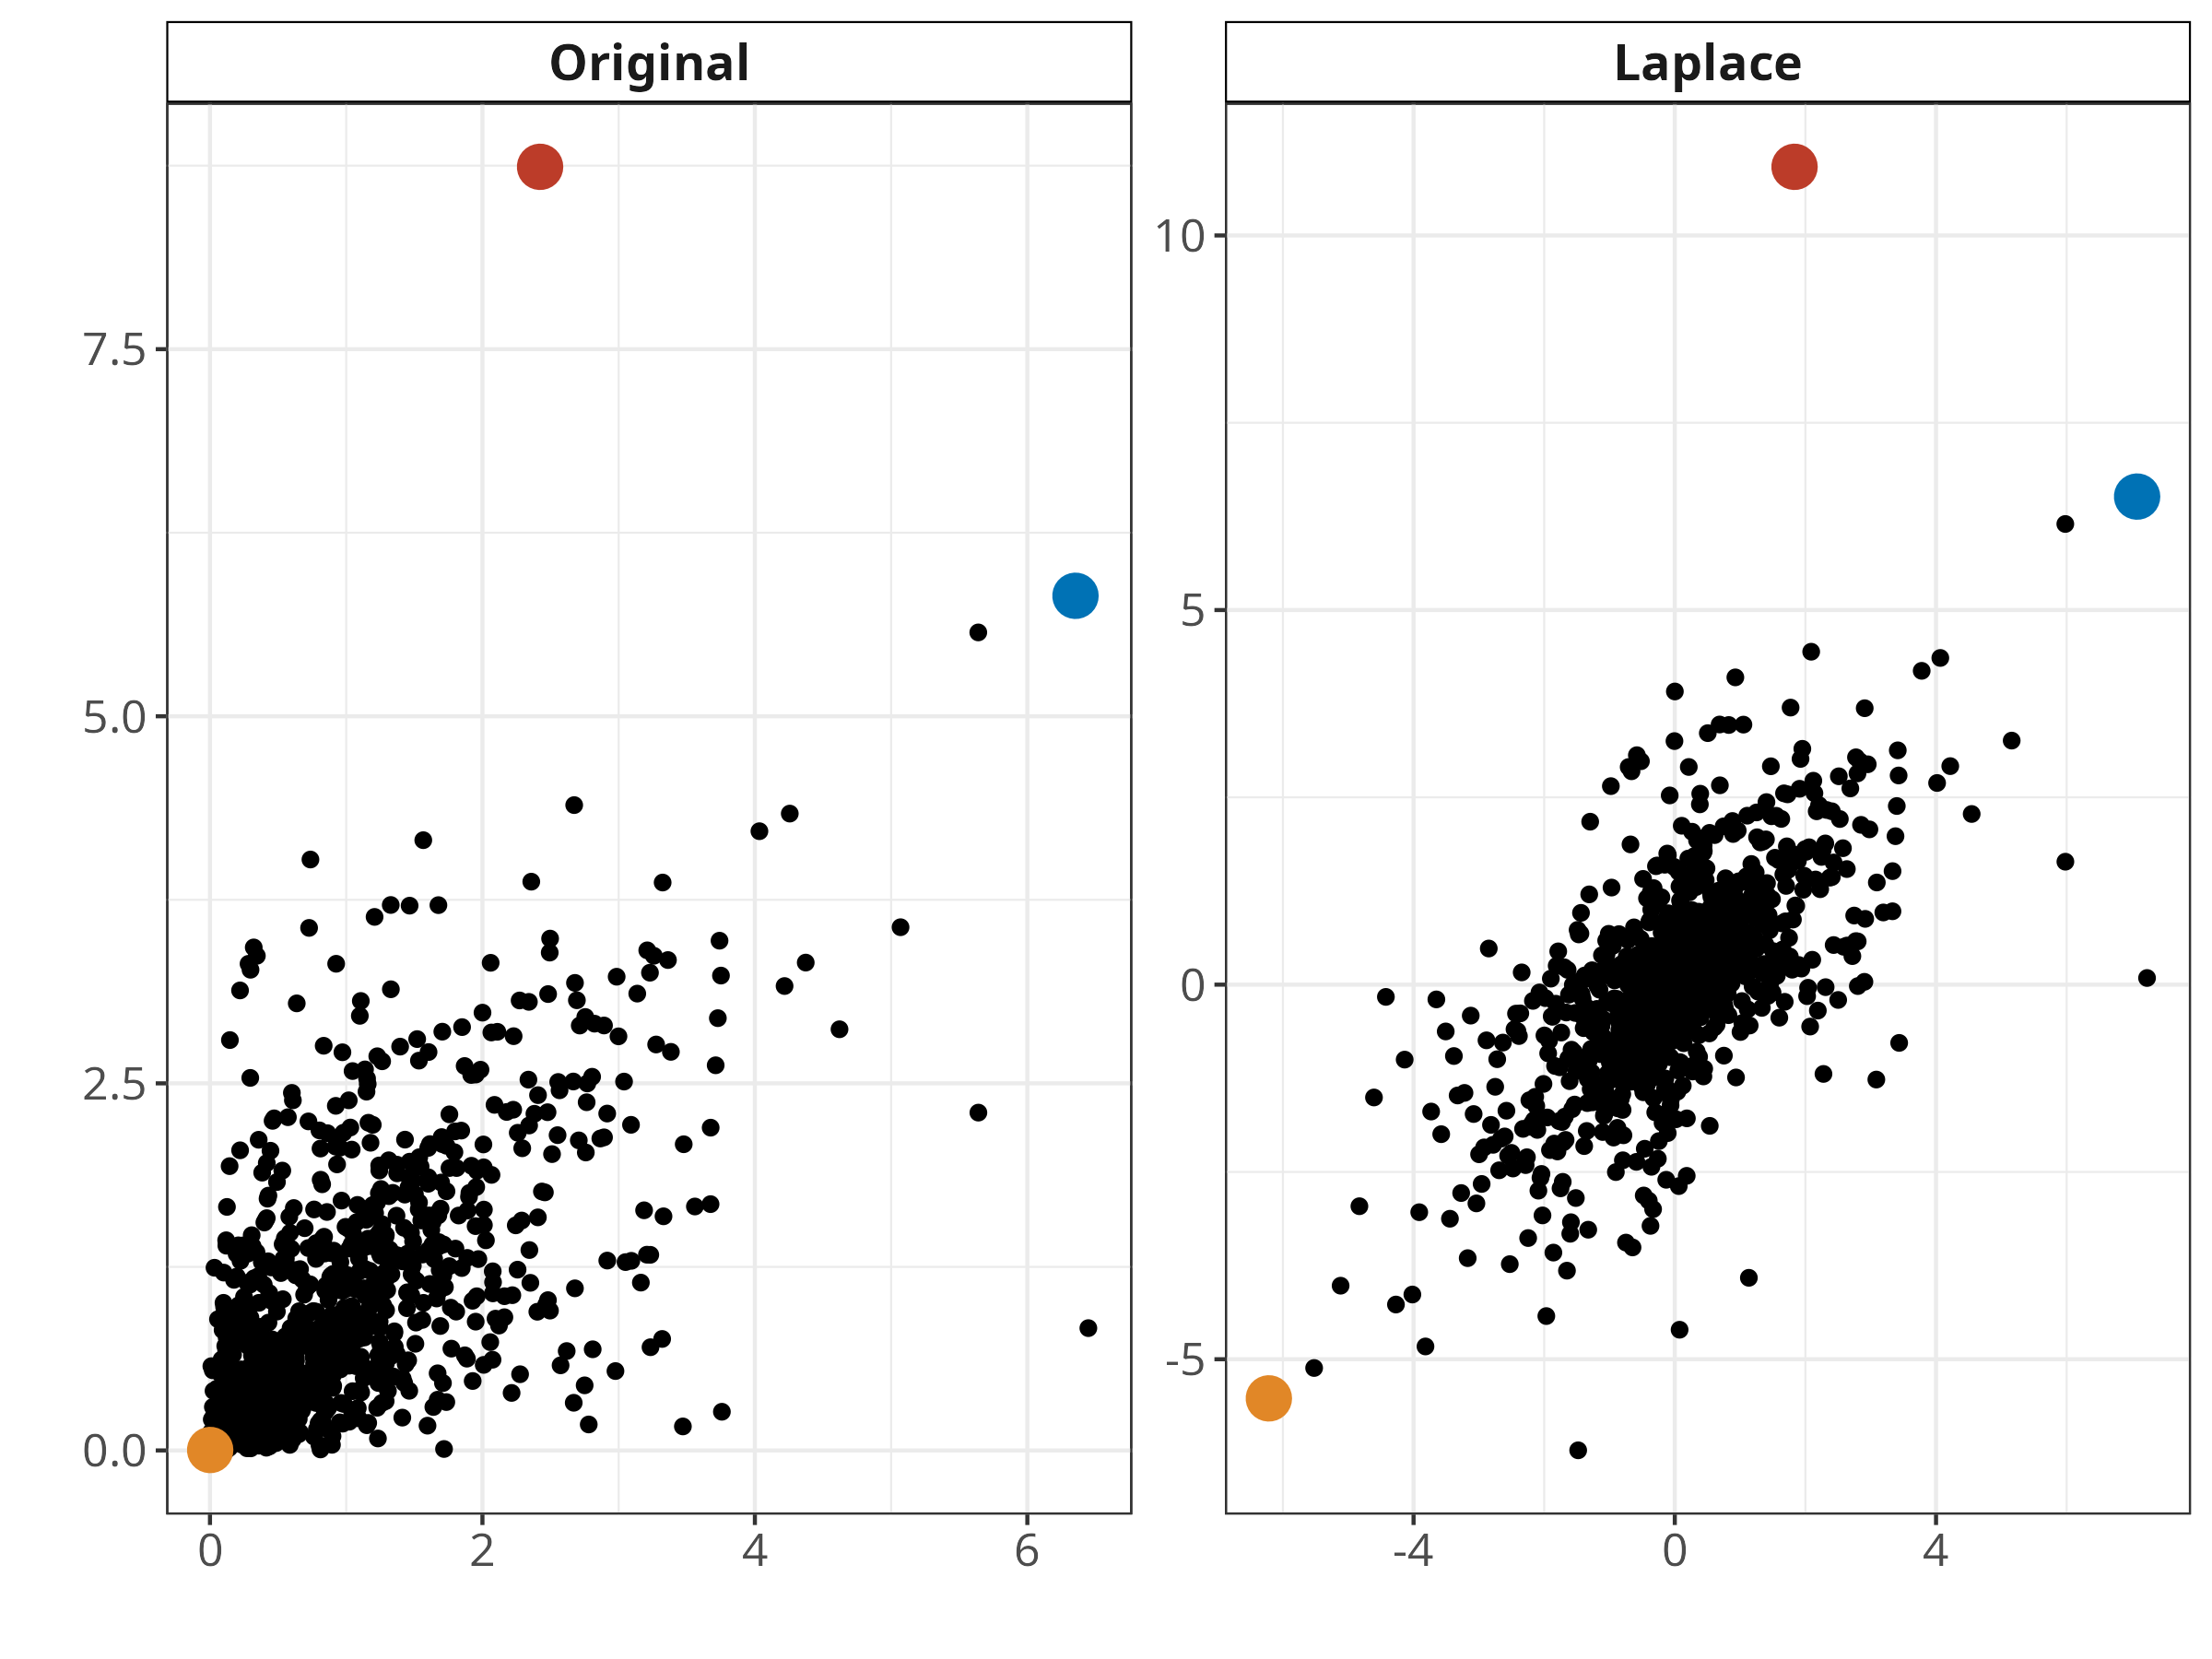
\includegraphics[width=1\textwidth]{plots/transform.png} 
\end{frame}

% Multivariate piecewise function, Z, Y independent
\begin{frame}{Dependence}
Dependence model:
\begin{equation*}
    \bm{Y}_{-i} = \bm{\alpha}_{\mid i}\bm{y}_i + \bm{y}_i^{\bm{\beta}_{\mid i}}\bm{Z}_{\mid i}, \text{ for } Y_i = y_i, y_i > u_{Y_i}.
\end{equation*}
\begin{itemize}
    \vspace{-8mm}
    \item $\alpha_{j \mid i} \in [-1, 1]$ is slope parameter for $Y_j$ conditional on $Y_i$.
    \item $\beta_{j \mid i} \in (-\infty, 1]$ is ``spread'' parameter, $\bm{\beta}_{\mid i}$ controls level of stochasticity in relationship between $\bm{Y}_{-i}$ and large $Y_i$. \todo{Power law??}
    \item Key assumptions: 
      \begin{itemize}
        \item Residuals $\bm{Z}_{\mid i} \sim N(\mu_i, \sigma_i)$, 
        \item $Z_{j \mid i}$ independent of large $Y_i$.
      \end{itemize}
    \item Special cases:
    \begin{itemize}
        \item $\bm{\alpha}_{\mid i} = 0, \bm{\beta}_{\mid i} = 0 \implies \bm{Y}_{-i}, \bm{Y}_{i}$ independent
        \item $\bm{\alpha}_{\mid i} = -1/1, \bm{\beta}_{\mid i} = 0 \implies$ perfect positive/negative dependence
        \item $-1 < \bm{\alpha}_{\mid i} < 1 \implies$ asymptotic independence \todo{Need to define above}
    \end{itemize}
\end{itemize}
\end{frame}

% \begin{frame}{Limitations}
%   \begin{itemize}
%     \item CE model is very flexible and can model all forms of extremal dependence, but can be difficult to fit.
%     \item Interpretation can sometimes be difficult due to estimating two parameters. 
%     \item CE often has large uncertainty in parameter estimates.
%     \item This is especially true when there are few observations of extreme events, which are rate by definition. 
%     \item How can we seek to overcome this?
%     % \item This is because the model is not identifiable, as parameters may not be unique.
%     % \item This means that the model can be fitted to the data in many different ways, leading to large uncertainty in parameter estimates.
%   \end{itemize}
% \end{frame}

\begin{frame}{Inference}
  \begin{itemize}
    \item Inference on $\bm{Y}_{-i} \mid Y_i$ done by conditioning on the exceedance of a high threshold $u_{Y_i}$ by $Y_i$.
    \item We assume this conditional distribution follows a diagonal multivariate Normal (MVN) distribution: 
      \begin{equation*} \label{eq:ce_norm}
        \bm{Y}_{-i} \mid Y_i = y_i \sim N\left(\bm{\alpha}_{\mid i} y_i + y_i^{\bm{\beta}_i} \bm{\mu}_{\mid i}, y_i^{\bm{\beta}_i} \bm{\sigma_{\mid i}}\right), Y_i > u_{Y_i}.
      \end{equation*}
    \item Therefore, \textbf{in comparing the dependence structure of multiple locations, we are essentially comparing the similarity between their respective MVN distributions}.
\end{itemize}

\end{frame}

\section{Clustering}

\begin{frame}{Clustering}
    \begin{itemize}
        \item CE is very flexible and conceptually simple, but can be difficult to fit, with large estimation uncertainty and difficult interpretations for parameters.
        \item There are extensions to CE model which seek to overcome shortcomings of ``vanilla'' model, such as spatial and spatio-temporal versions.
        \item Alternative/additional approach: \textbf{clustering}
        \item Clustering done for two main reasons: 
          \begin{itemize}
            \item \textbf{to enhance the explainability and interpretation of data},
            \item to improve parameter estimation.
          \end{itemize}
        \item \textbf{How best to cluster for CE model?}
    \end{itemize}
\end{frame}

\begin{frame}{Kullback-Leibler divergence}
  The Kullback-Leibler (KL) divergence between two continuous distributions $P$, $Q$ is given by
  \[
    KL(P \mid\mid Q) = \int_{-\infty}^{\infty} p(y) \log\left(\frac{p(y)}{q(y)}\right) dy.
  \]
  \vspace{-5mm}
  \begin{itemize}
  \item For two MVNs, the KL divergence has closed form. 
  \item However, KL divergence is asymmetric ($KL(P \mid\mid Q) \ne KL(Q \mid\mid P)$) and not a ``true'' metric, making it a poor choice as measure of dissimilarity for clustering. 
  \end{itemize}
\end{frame}

\begin{frame}{Jensen-Shannon divergence}
  \begin{itemize}
    \item The Jensen-Shannon divergence is given by
      \[
        JS(P \mid\mid Q) = \frac{1}{2} KL(P \mid\mid M) + \frac{1}{2} KL(Q \mid\mid M),
      \]
      where $M = \frac{1}{2}(P + Q)$ is a mixture distribution.
    \item JS is symmetric and a true metric!
    \item However, the mixture of two normals is non-normal \\ $\implies$ no closed form for two MVNs. 
  \end{itemize}
\end{frame}

\begin{frame}{skew-geometric Jensen-Shannon divergence}
\begin{itemize}
  \item Instead, we can use the weighted geometric mean $G_{\alpha}(x, y) = x^{\alpha} y^{1 - \alpha}, \alpha \in [0, 1]$
  \item The weighted product of two members of the same exponential family also comes from this family, so we will have another multivariate normal. 
  \item From this, we define the \textbf{skew-geometric Jensen-Shannon divergence}
    \[
      JS^{G_{\alpha}}(P \mid\mid Q) = \frac{1}{2} KL(P \mid\mid G_{\alpha}(P, Q)) + \frac{1}{2} KL(Q \mid\mid G_{\alpha}(P, Q))
    \]
  \item This has both closed form and for MVNs and is a true metric, making it a good candidate as a dissimilarity measure for clustering. 
  \item Sensible choice is $\alpha = 0.5$. %, may adapt data-driven or theoretically motivated approach in the future. 
\end{itemize}
\end{frame}

\begin{frame}{Partitioning Around Mediods}
  \begin{itemize}
    \item Now we have a dissimilarity measure, we can use it to cluster the data.
    \item We use the PAM algorithm, which is a partitioning clustering algorithm that uses the mediod of each cluster as the representative point.
    \item Cluster centres are actual data points, making them more interpretable than the centroids of k-means, especially for spatial and spatio-temporal applications. 
    \item Also, as we are clustering on functional space, advantageous to have actual set of CE parameters rather than some summary as cluster centre.
  \end{itemize}
\end{frame}

\begin{frame}{Selecting $k$ with total within cluster sum of squares \& elbow plot}
  \begin{itemize}
    \item \textbf{TWGSS}:
      \[
        \mathrm{TWGSS}(k)
        % = \sum_{i=1}^{k}\sum_{x \in C_i} d\bigl(x, m_i\bigr), d = JS^{G_{\alpha}}
        = \sum_{i=1}^{k}\sum_{x \in C_i} JS^{G_{\alpha}}\bigl(x, m_i\bigr),
      \]
    \item \textbf{Elbow Plot:} Plot $\mathrm{TWGSS}(k)$ vs.\ $k$ and observe the curve
    \item \textbf{Elbow Criterion:} Select $k^*$ at the “elbow” where TWGSS reduction sharply slows
  \end{itemize}

  \vspace{0.5em}
  \begin{center}
    
\includegraphics[width=0.7\textwidth]{plots/elbow_plot.png}
  \end{center}
\end{frame}

\section{Simulations}

\begin{frame}{Simulation Study}
  \begin{itemize}
    \item We perform a simulation study to assess the performance of our clustering algorithm.
    \item Generate data for multiple ``locations'', each with their own specified dependence structure.
    \item Can generate known ``clusters'' by specifying locations to have similar dependence structures.
    \item We evaluate our clustering solution using the Adjusted Rand Index, and reduction in uncertainty using bootstrapping.
  \end{itemize}
\end{frame}

\begin{frame}{Gaussian Copula}
  \begin{itemize}
    \item For a single location, generate multivariate data from bivariate Gaussian copula, where dependence controlled by $\rho_{Gauss}$ (off-diagonals of $\Sigma$). 
    \item \cite{Keef2013} shows that for bivariate Gaussian copula, the asymptotic CE parameters are $\alpha = \rho_{\text{Gauss}}^2, \beta = 1/2$, so we can compare estimated parameters to true asymptotic values. 
    % \item Sample from copula, transform to Laplace margins and use CE to estimate bivariate extremal dependence structure at this location.
    \item Can cluster locations using $JS^{G_{\alpha}}$ dissimilarity measure between CE fits at each location.
    \item Example: Generated 12 locations with 1000 observations of 2 variables
    \item 3 clusters of 4 locations each.
  \end{itemize}
\end{frame}

\begin{frame}{Gaussian Copula - results}
  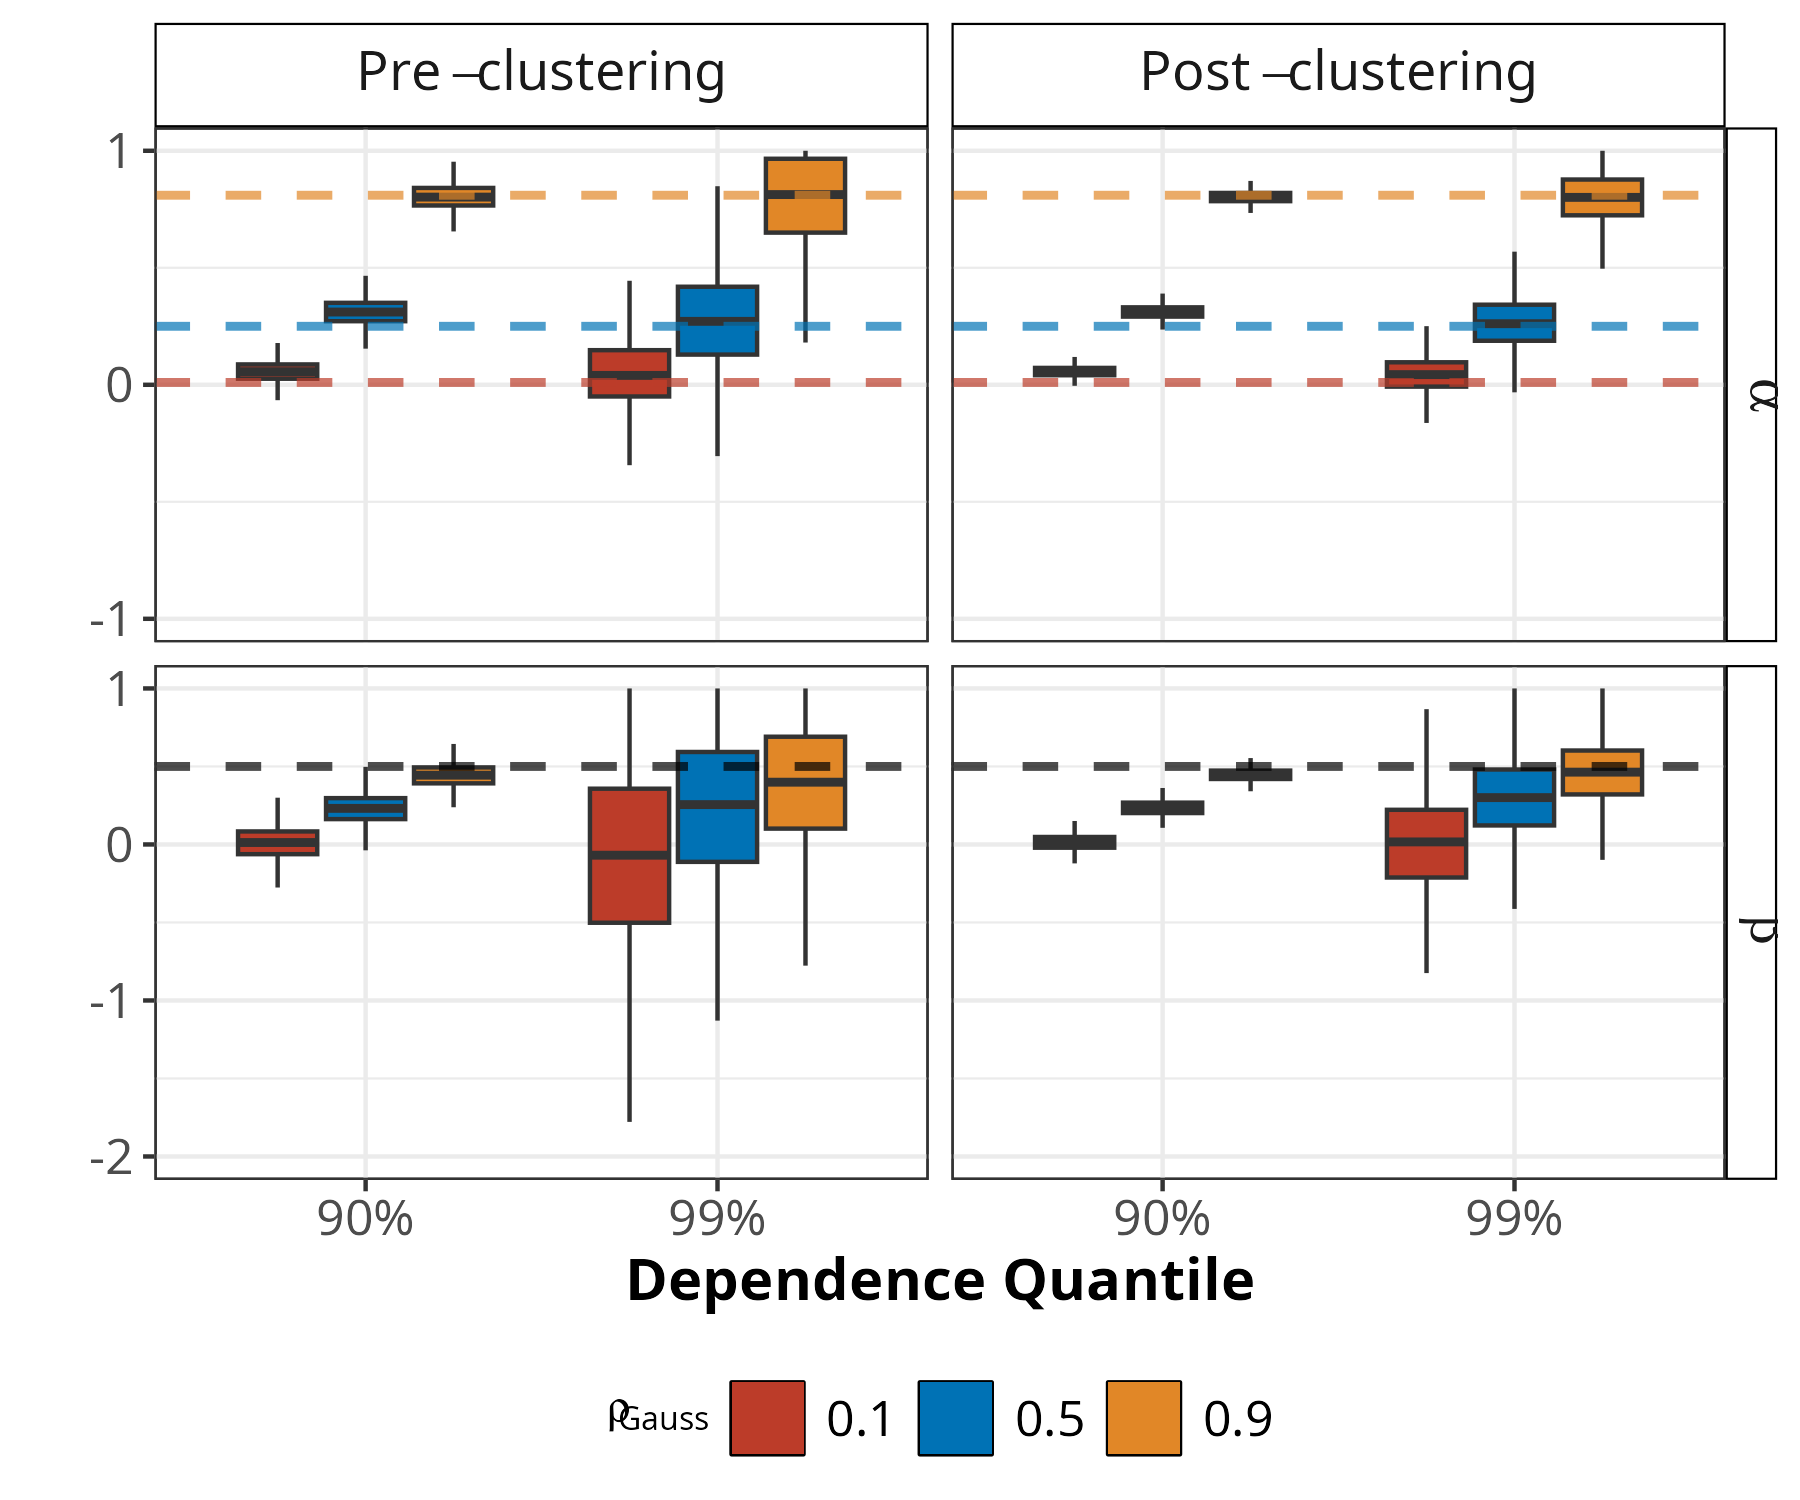
\includegraphics[width=0.9\textwidth]{plots/sim_01_gauss_cop.png}
\end{frame}

\begin{frame}{Mixture Simulation}
  \begin{itemize}
    \item Introduce data generated from mixture of Gaussian and t-copulas
    \item Idea: 
    \begin{itemize} 
      \item Gaussian copula generates observations exhibiting extremal independence, 
      \item the t-copula induces extremal dependence.
    \end{itemize}
    \item No theoretical guarantees for $\alpha, \beta$, but perhaps more realistic. 
    \item First, generated 12 locations with 1000 observations of 2 variables, now with 2 clusters of 6 locations each. 
    \item $\rho_{gauss} = 0.5$, grid search performed over $\rho_{t} \in [0, 1]$ for both clusters.
    \item Compared to performance of Vignotto clustering algorithm, which is the leading competitor in the bivariate setting \cite{Vignotto2021}.
  \end{itemize}
\end{frame}

\begin{frame}{Mixture Simulation (two variables)}
  \todo{Replace with plot once more samples have been used!}
  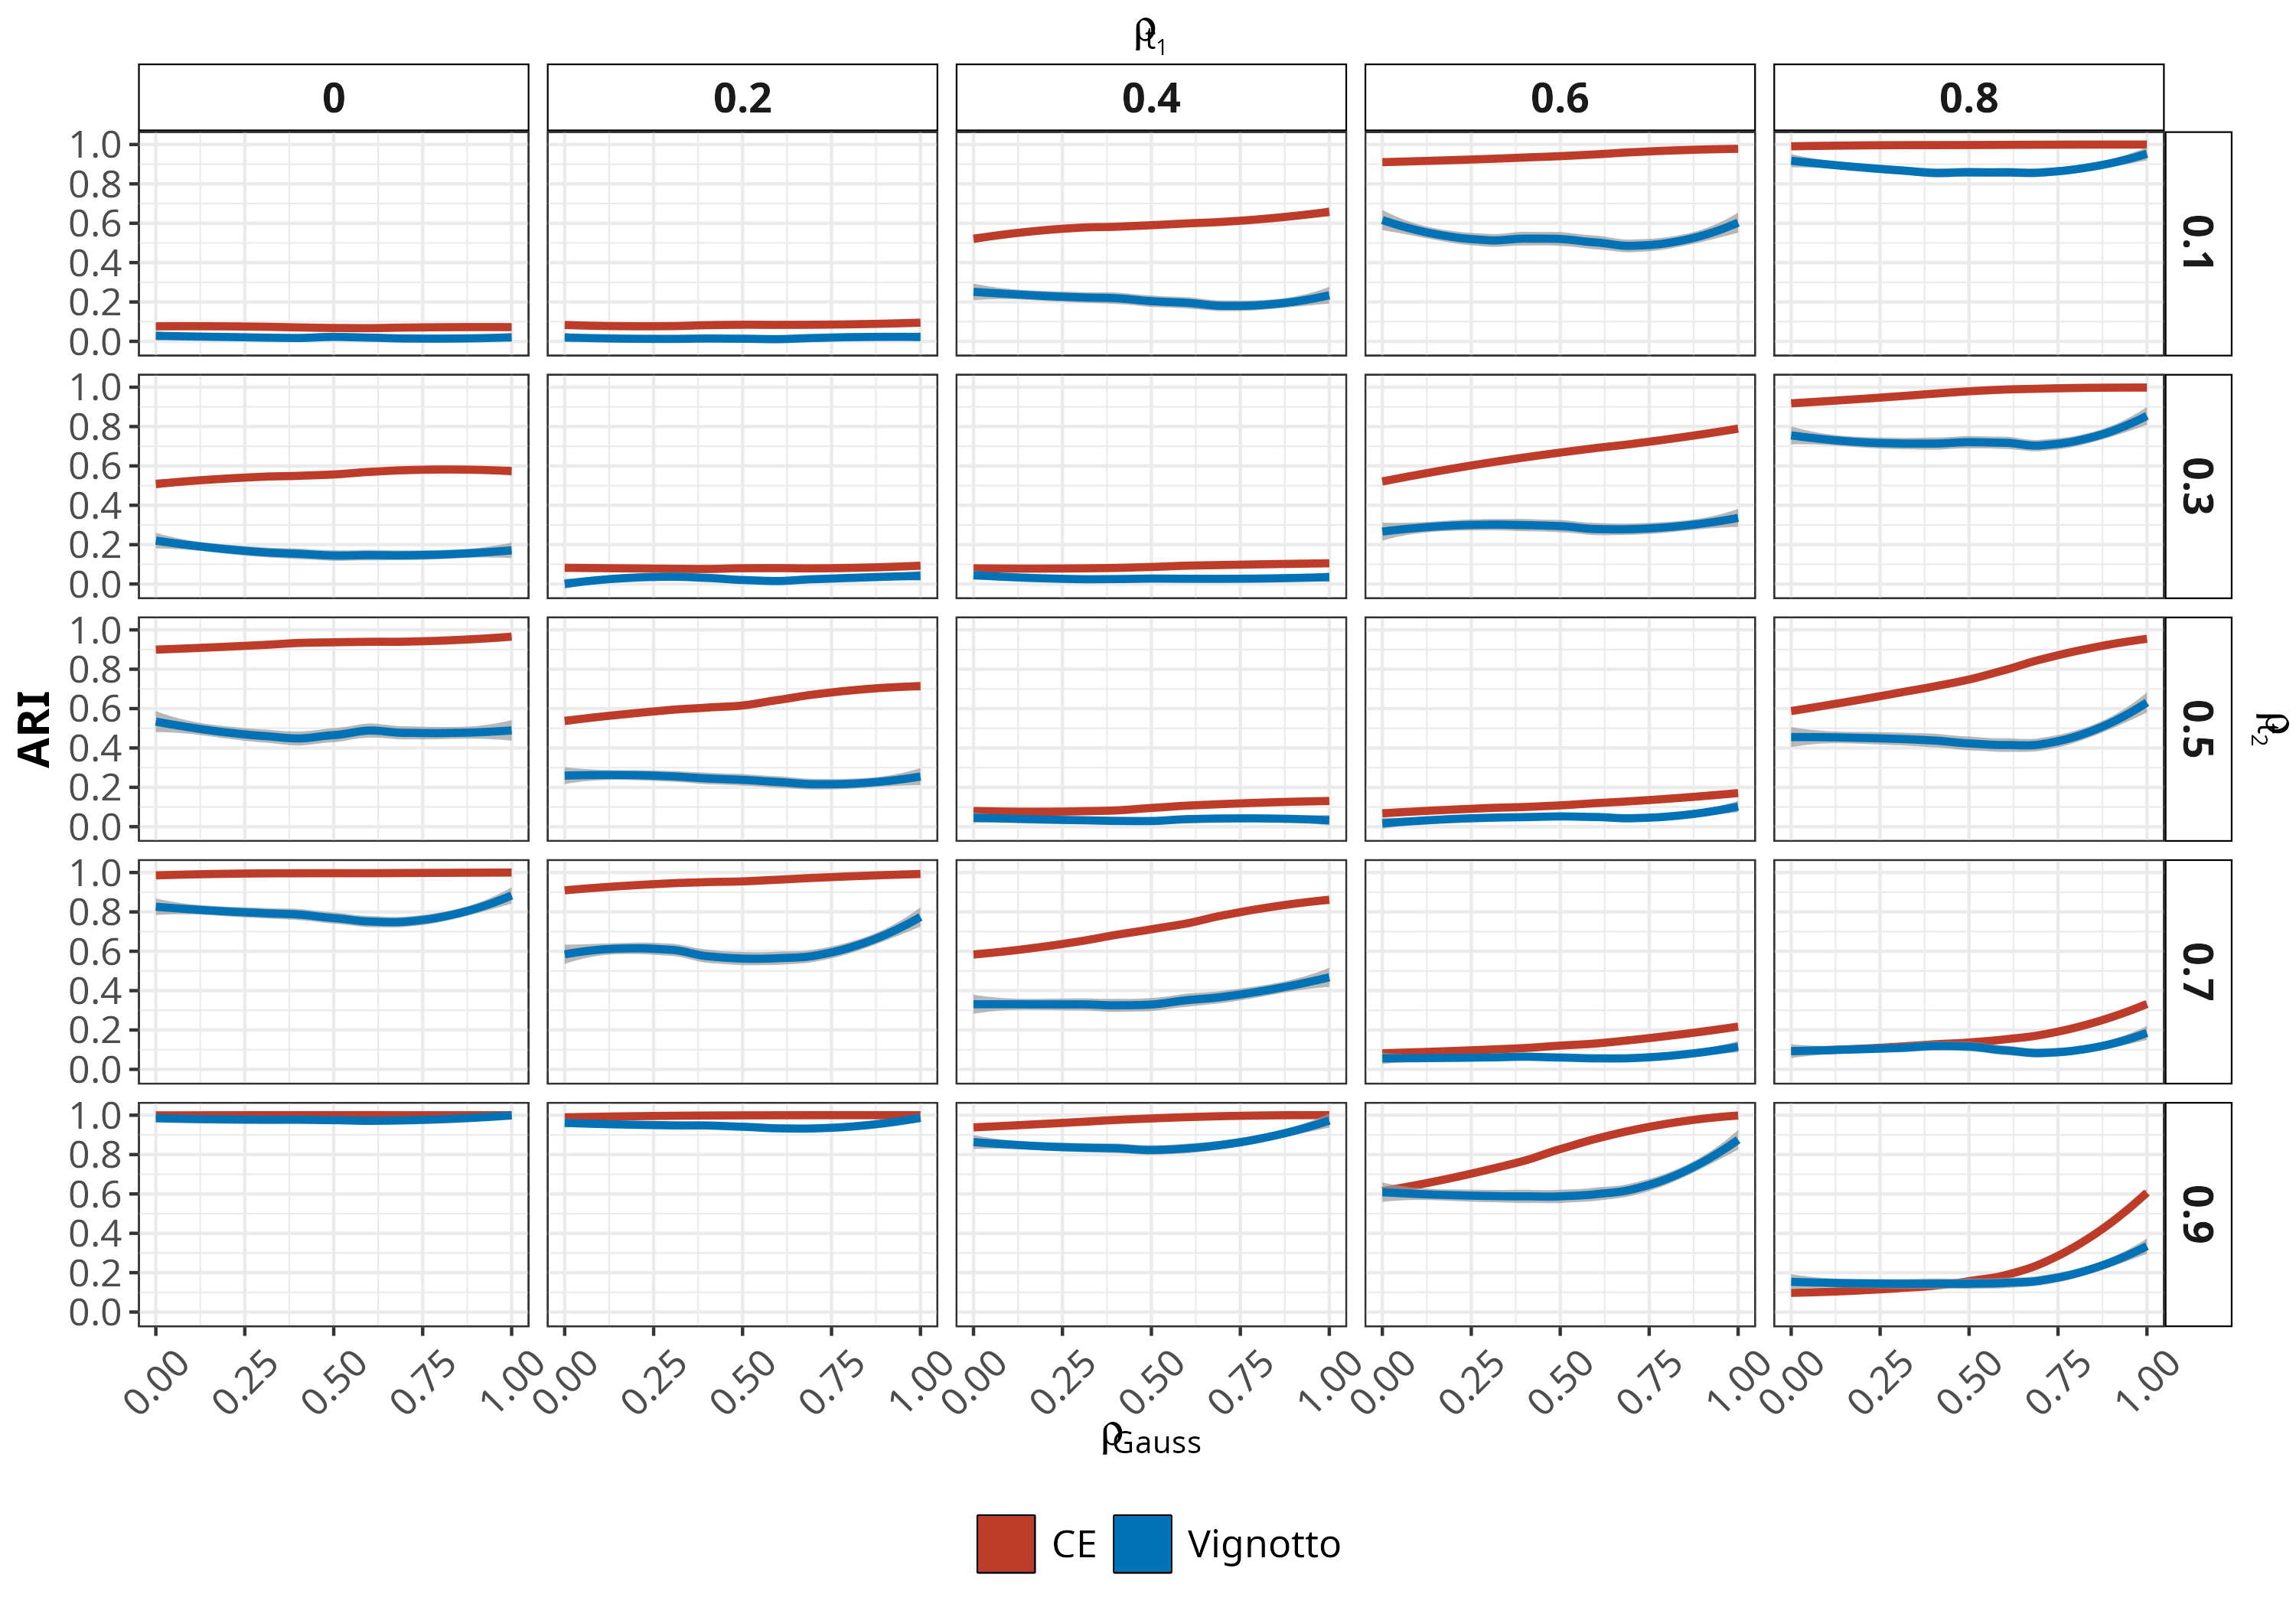
\includegraphics[width=1\textwidth]{plots/sim_01b_ce_vs_vi_dqu_0.9.png}
\end{frame}
% 

\begin{frame}{Other scenarios}
\begin{itemize}
  \item We also perform the same simulation study where three variables are
  available at each location, for which our clustering algorithm is uniquely applicable.
  \item Finally, we generate more ``realistic'' example with 60 locations with 
    three clusters of 30, 20 and 10 location each, to more closely mimic the Irish dataset. 
\end{itemize}
\end{frame}

\begin{frame}{Mixture Simulation (three variables)}
  \todo{Replace with plot once more samples have been used!}
  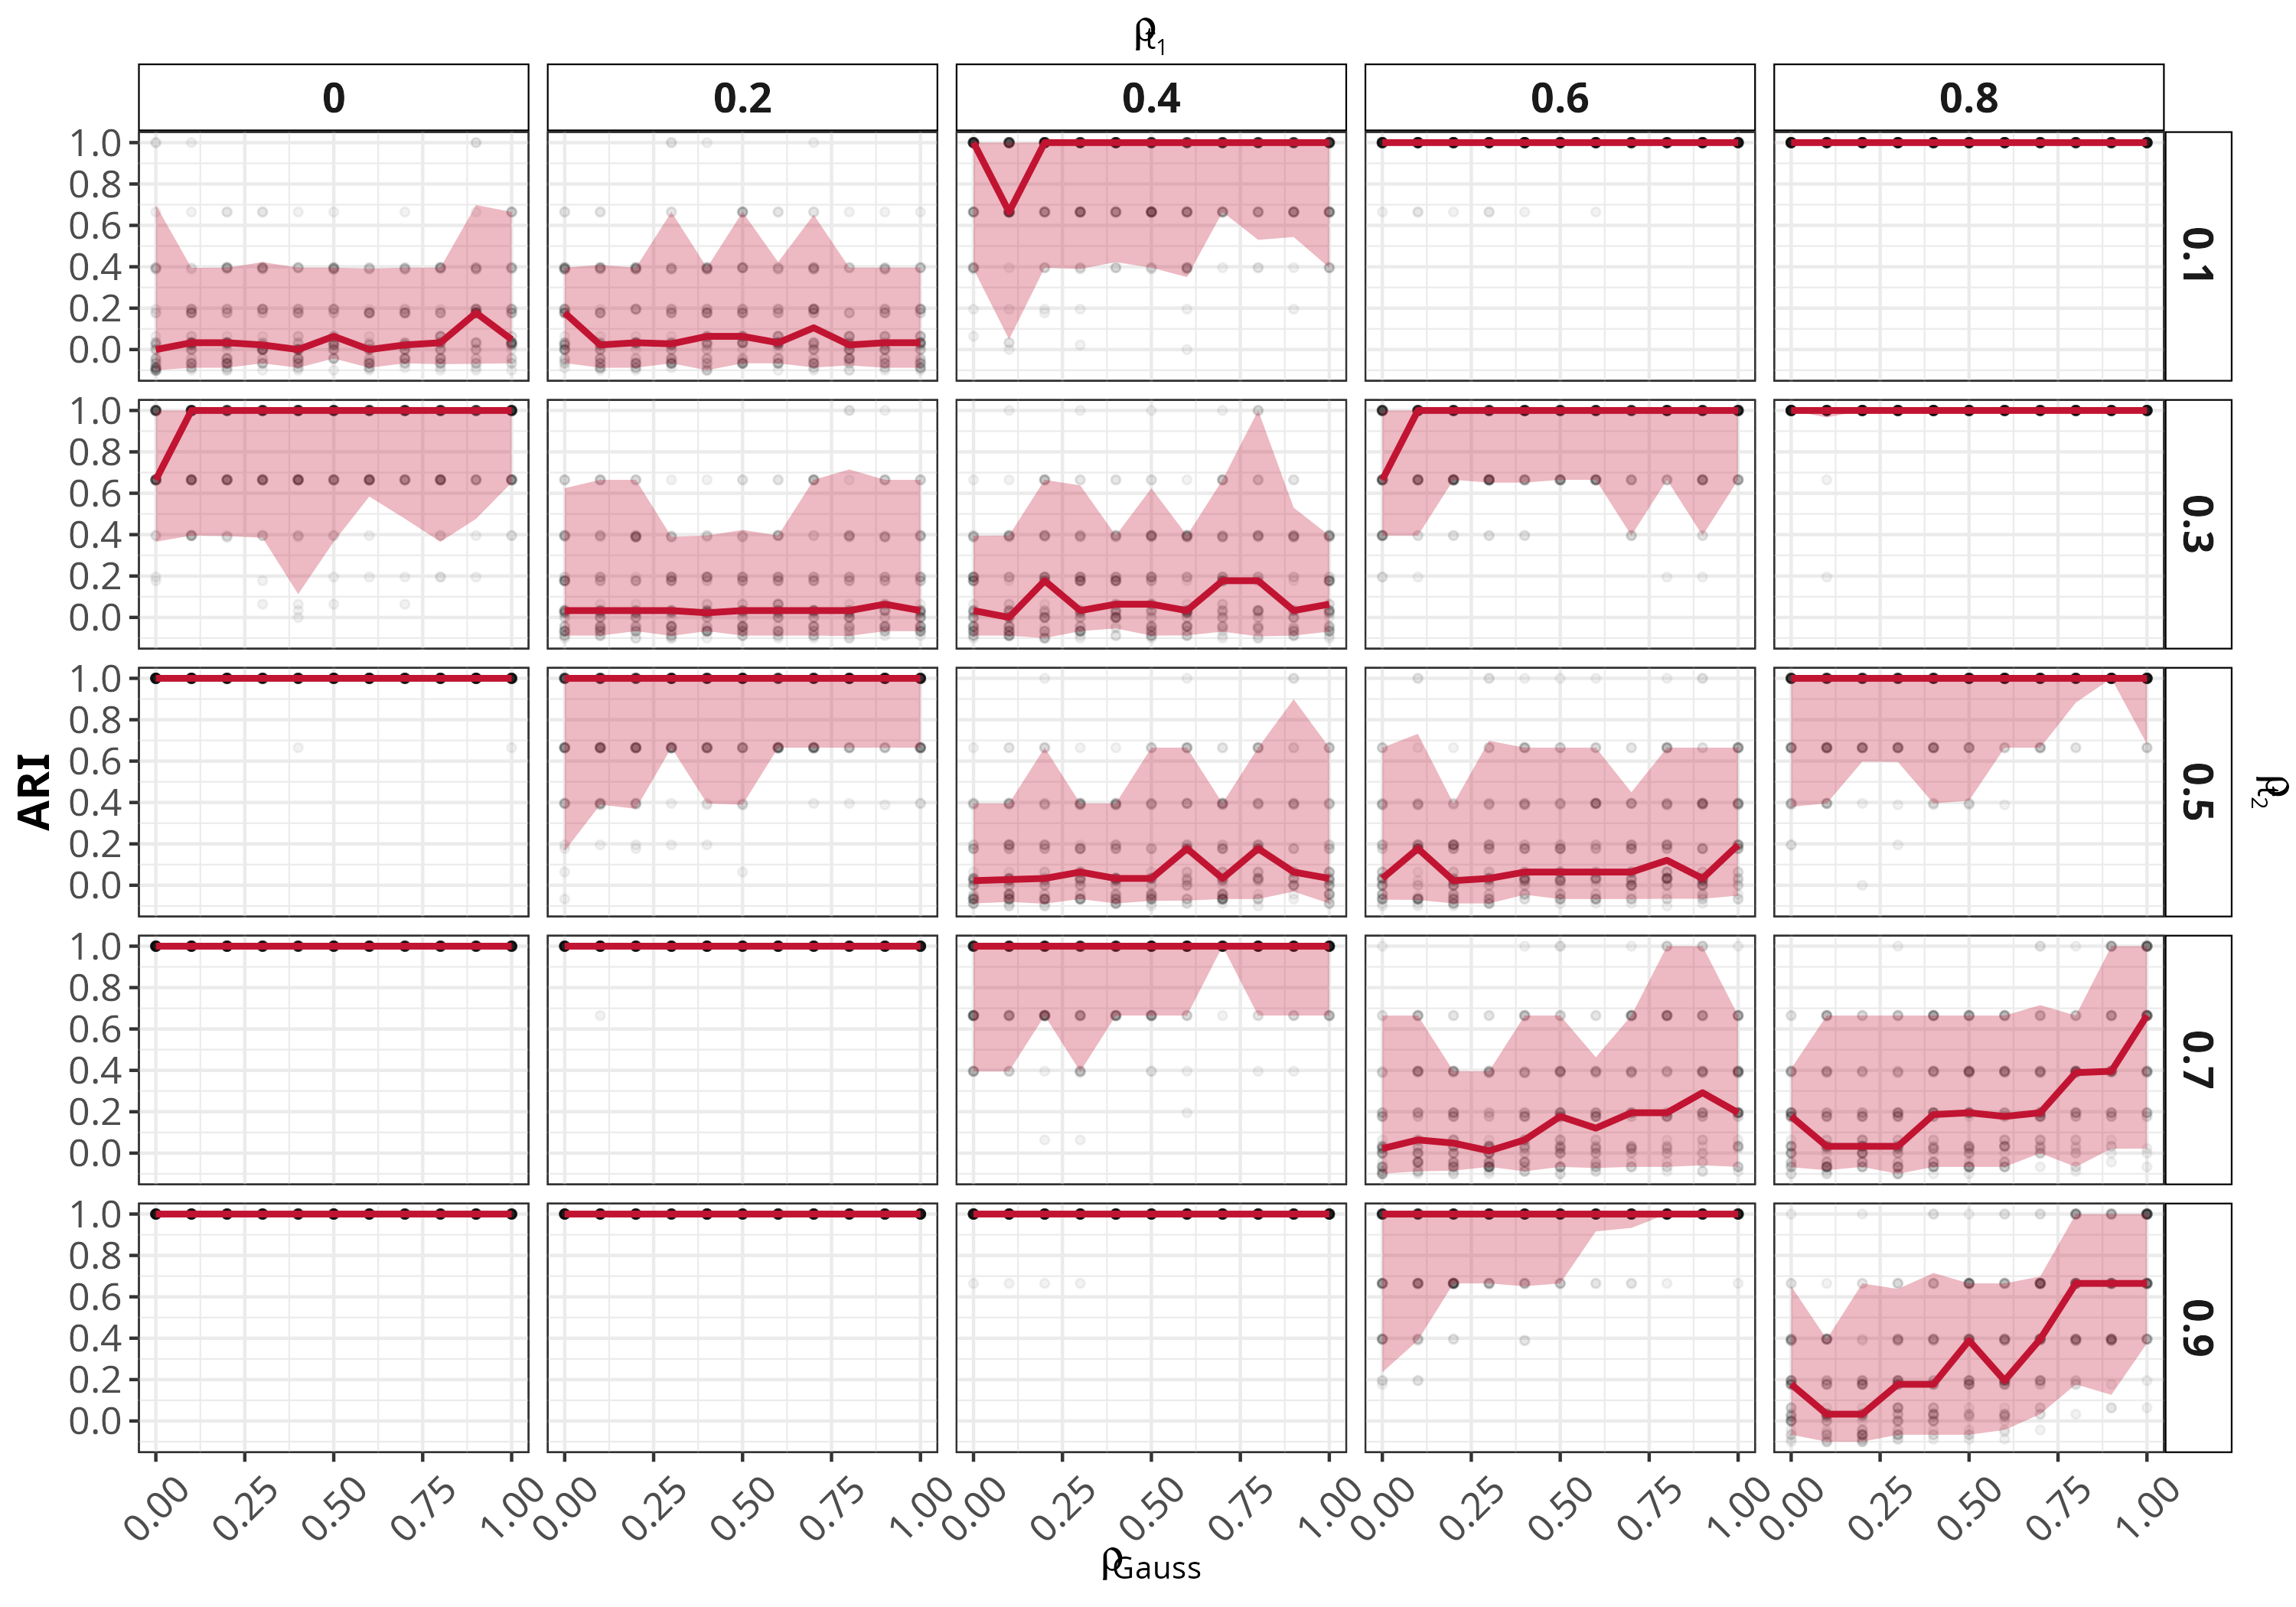
\includegraphics[width=1\textwidth]{plots/sim_01c_js_sens_3_var_dqu_0.9.png}
\end{frame}

\begin{frame}{More Realistic Example}
  \todo{Replace with plot once more samples have been used!}
  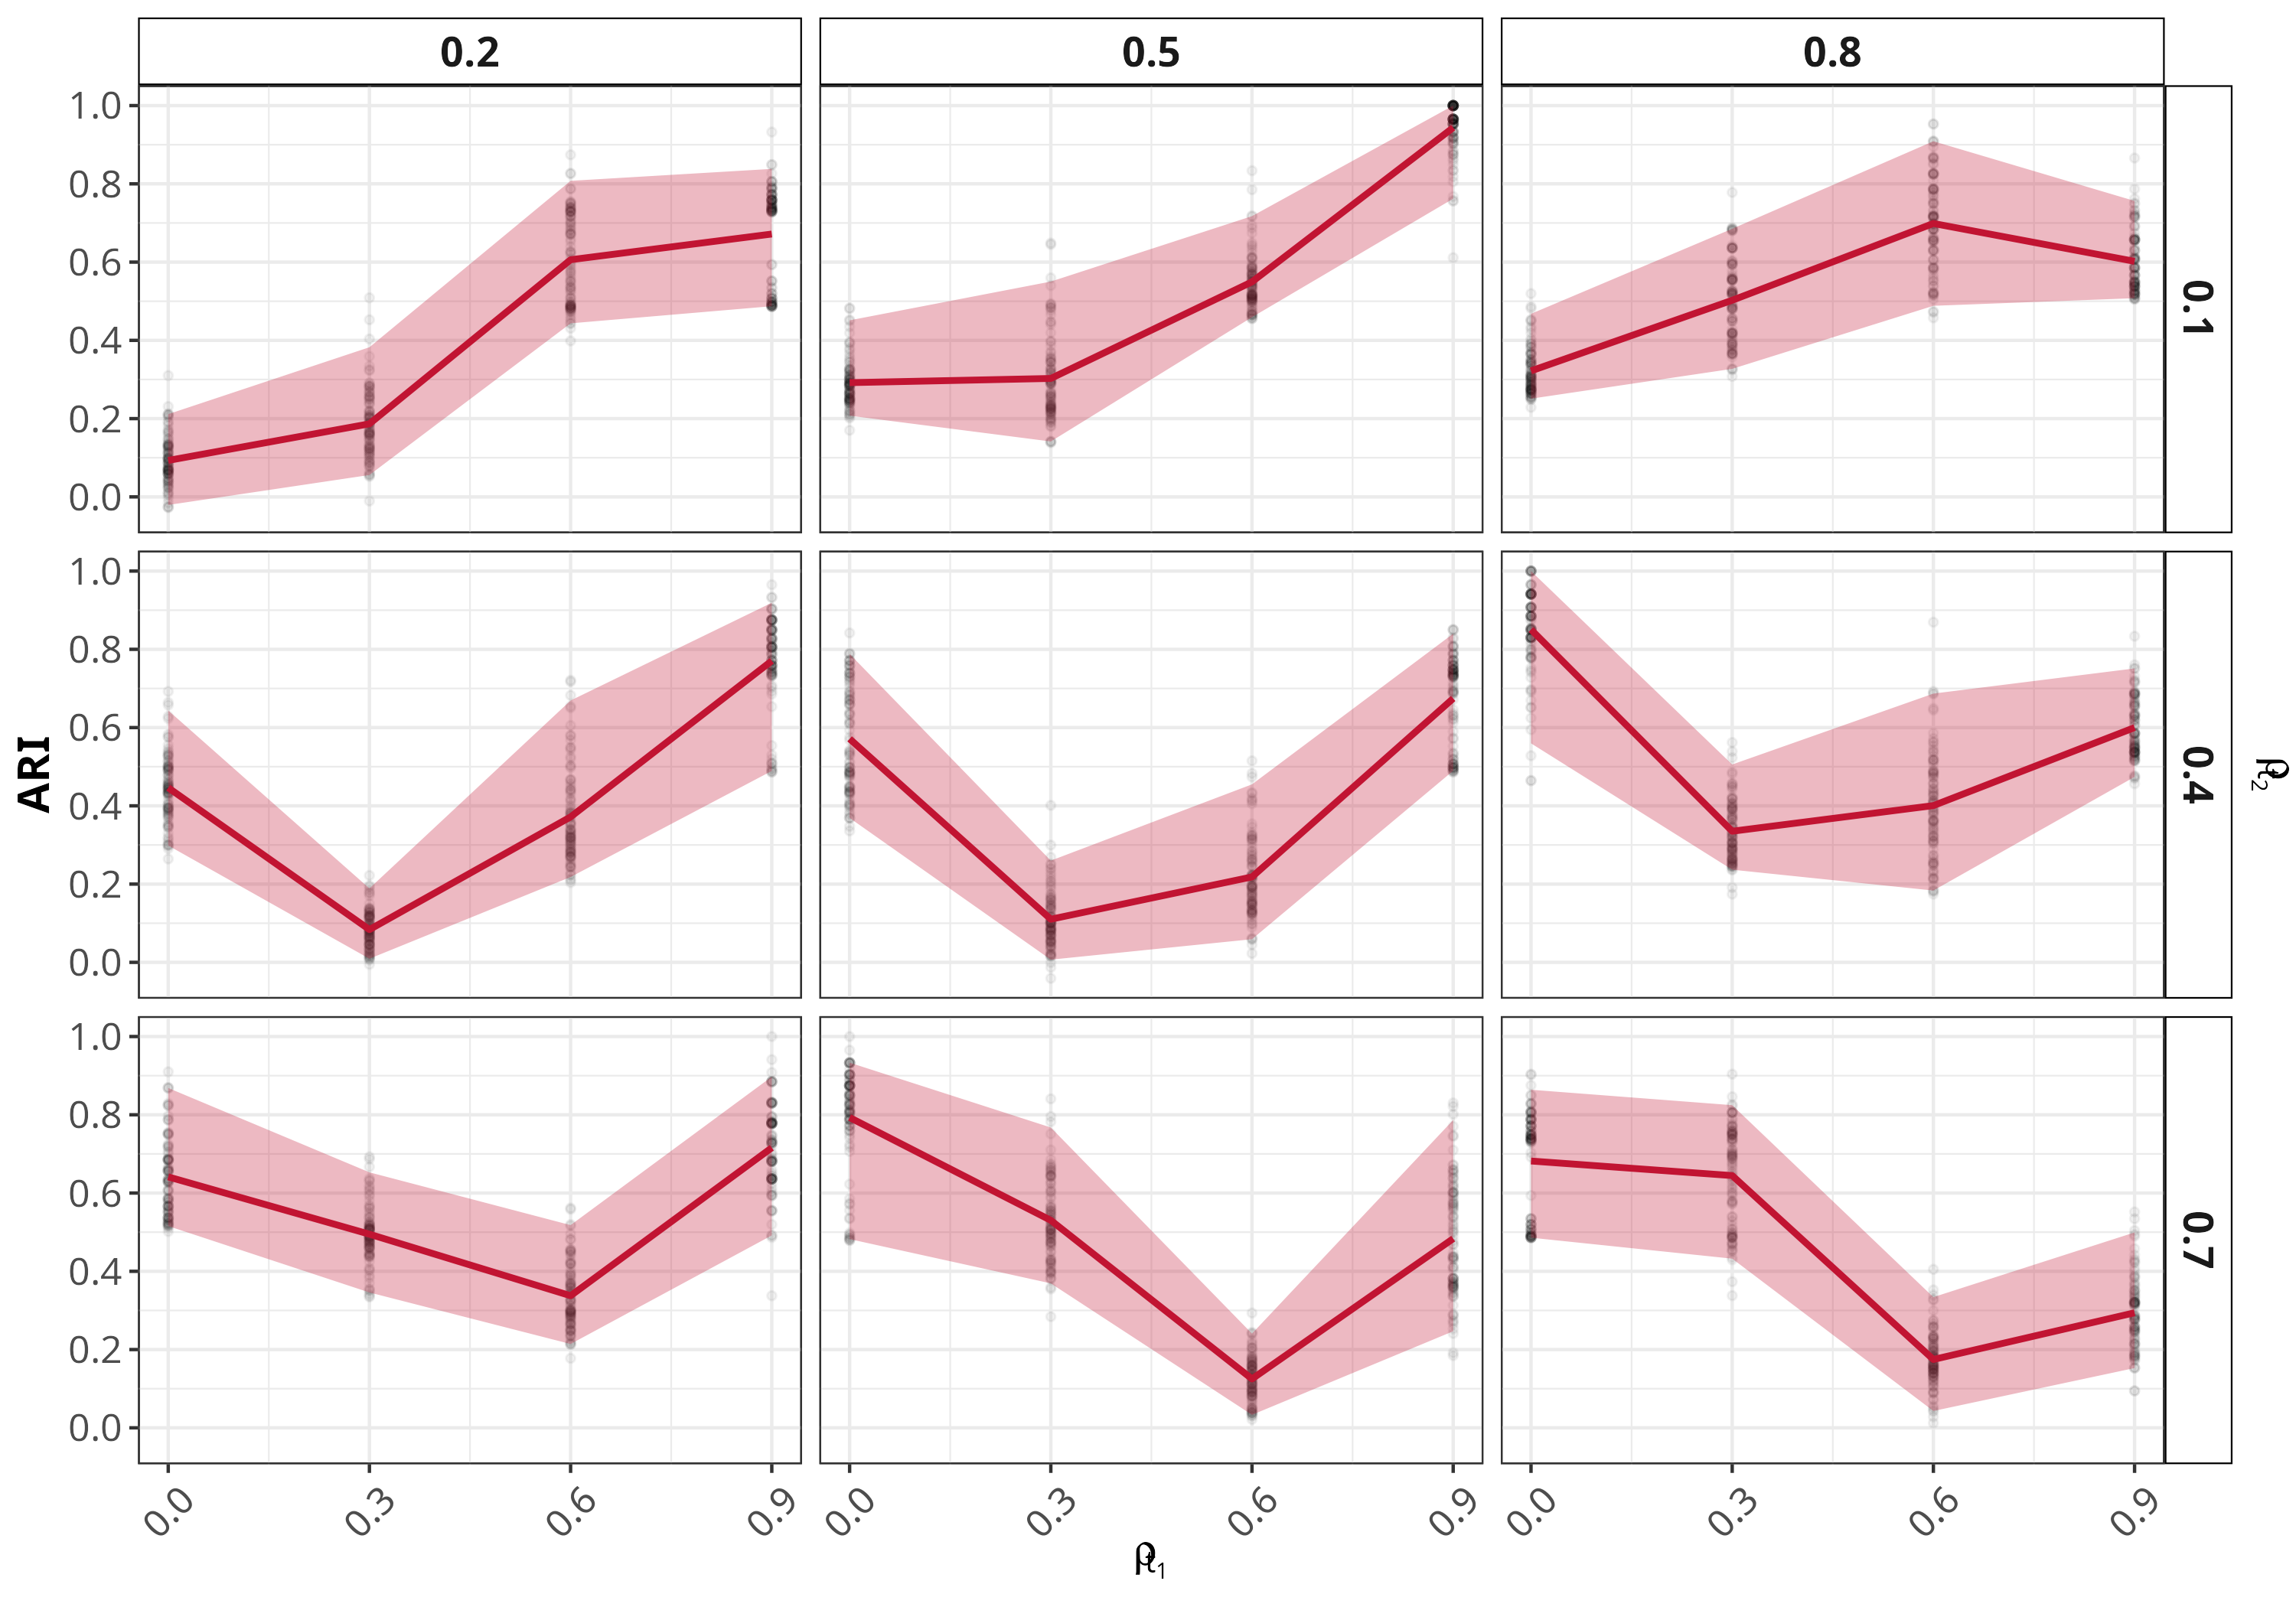
\includegraphics[width=1\textwidth]{plots/sim_01d_js_sens_3_var_dqu_0.9.png}
\end{frame}

% TODO Needed, as we're focusing on interpretability??
% \begin{frame}{Uncertainty Reduction}
%   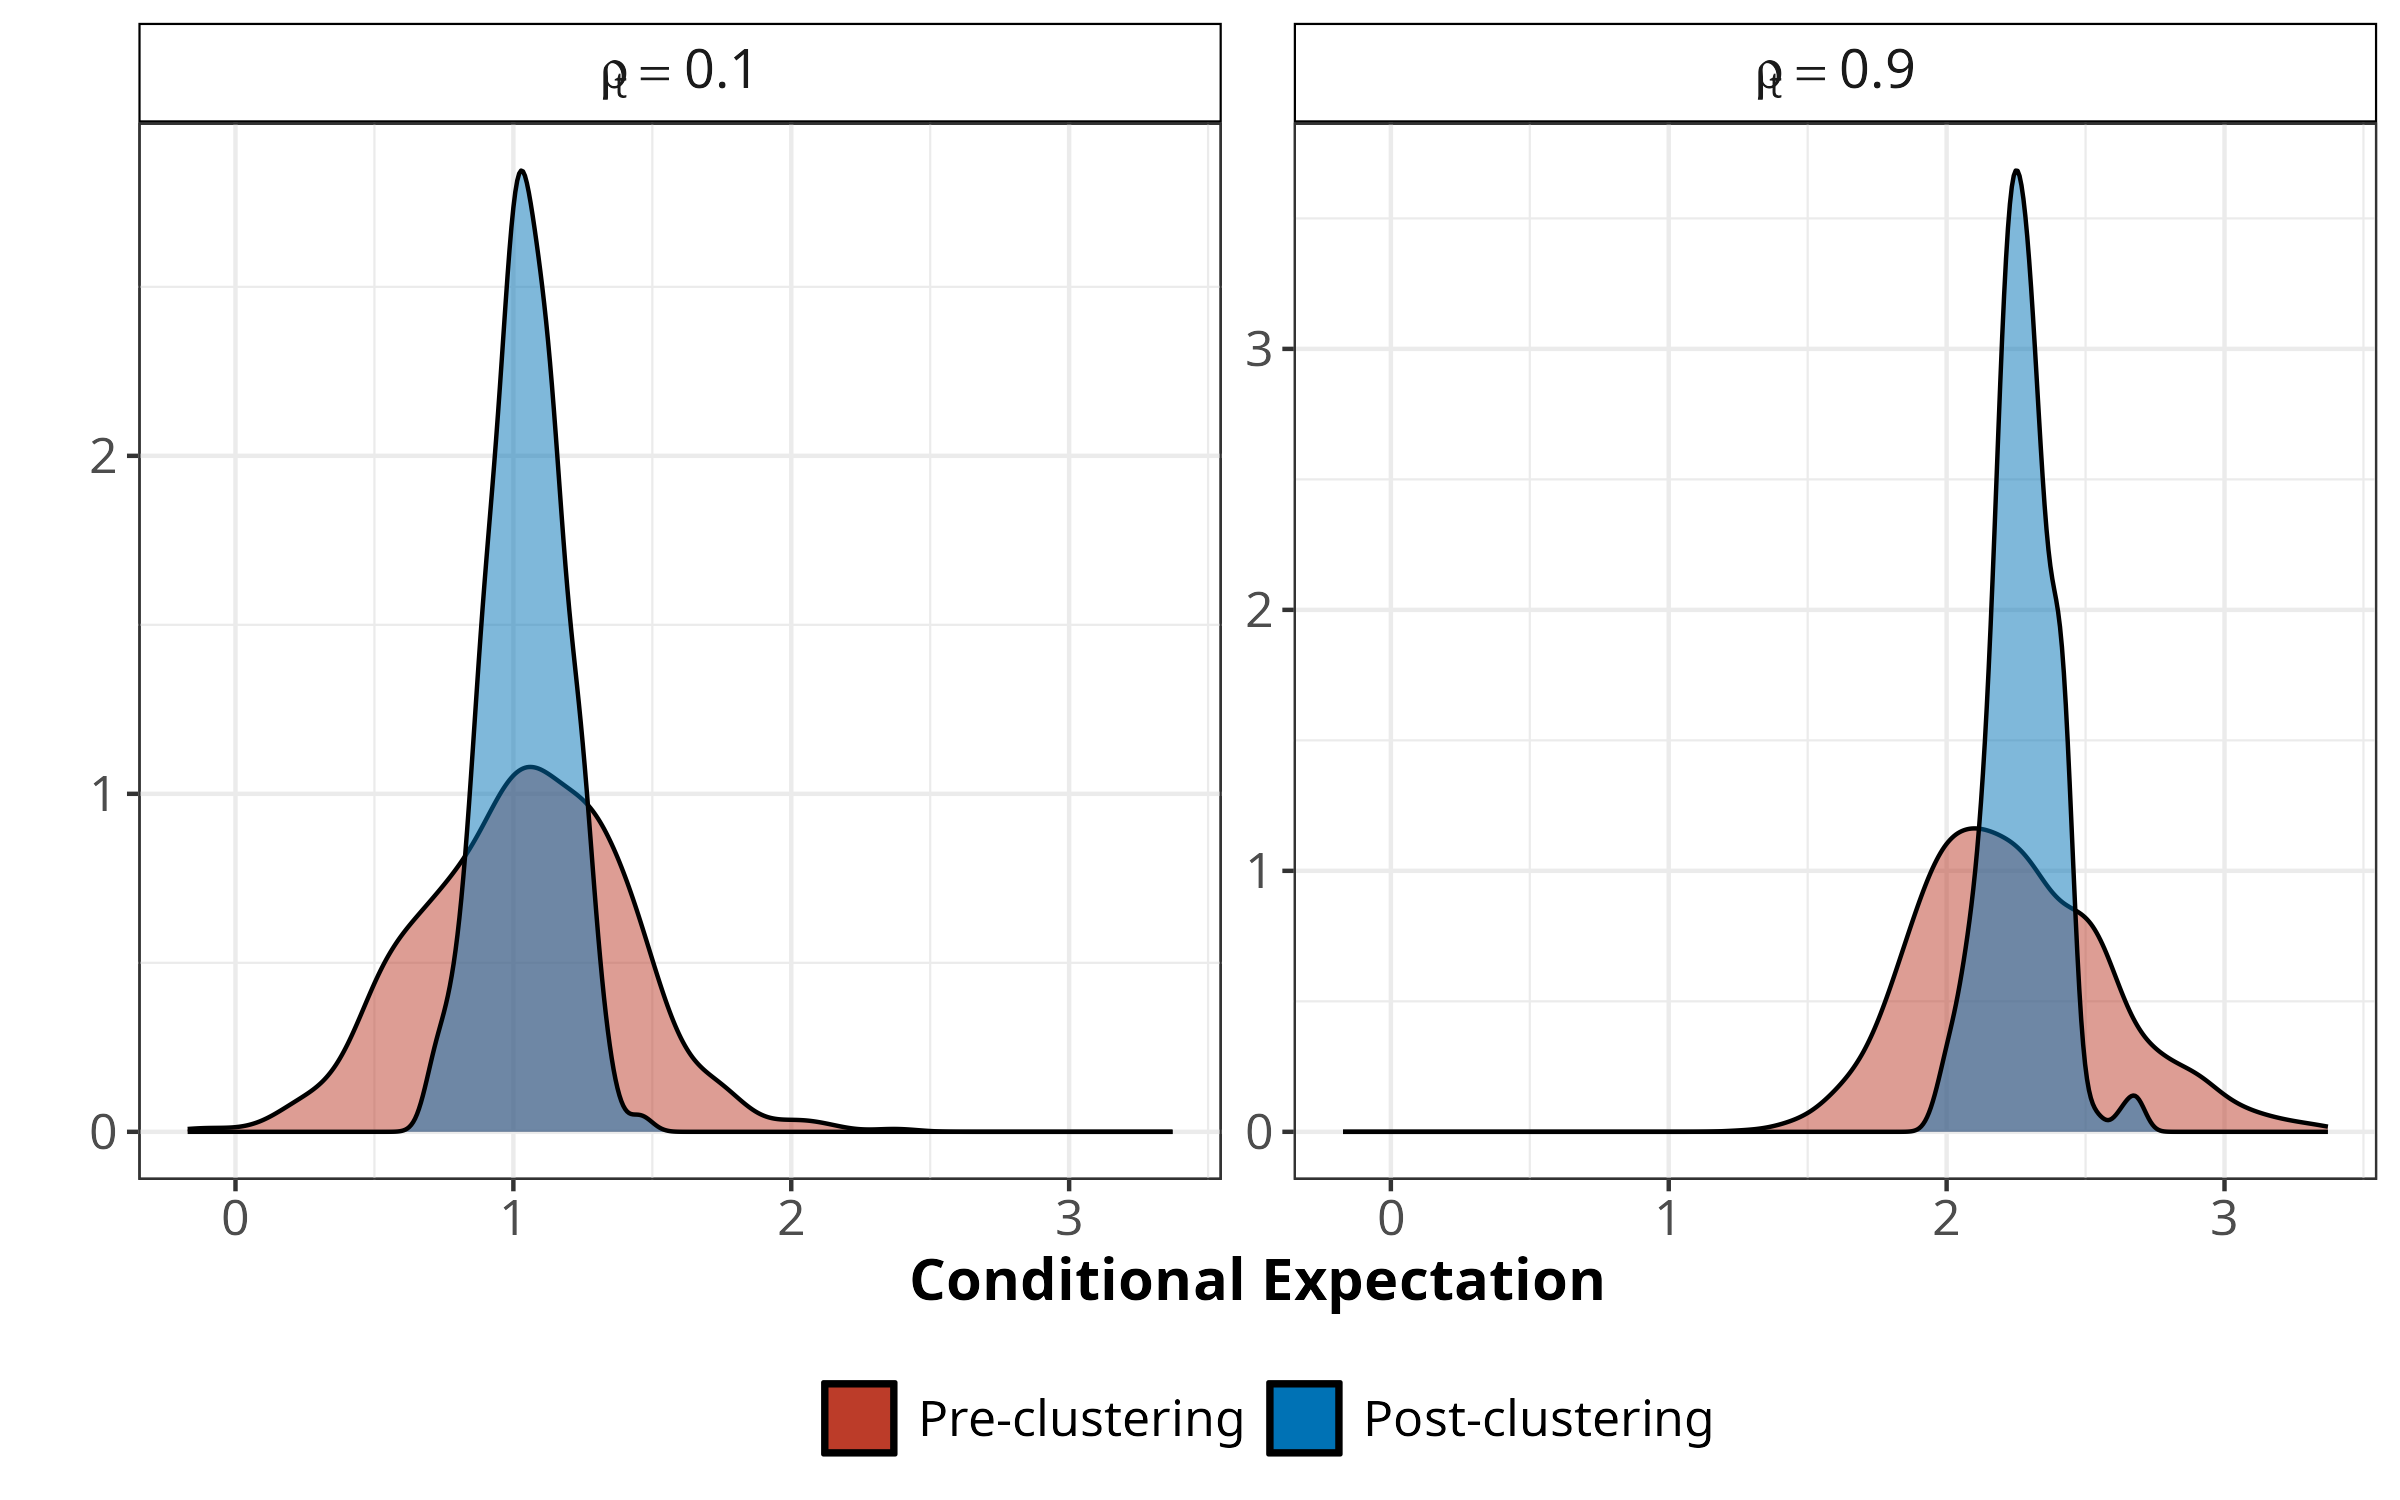
\includegraphics[width=1\textwidth]{plots/sim_01e_bootstrap.png}
% \end{frame}

\section{Motivating Example: Ireland Meteorological Data}

% Describe motivating example
\begin{frame}{Ireland}
  \begin{minipage}{0.45\textwidth}
      \begin{itemize}
          \item Precipitation and wind speed in Ireland, 1990-2020
          \item Precipitation data from 59 Met Éireann weather sites across country, wind data from ERA5 reanalysis dataset.
          \item Weekly sum of precipitation and mean of daily wind speed maxima for Winter only (Oct-Mar), in line with Vignotto \cite{Vignotto2021}. 
      \end{itemize}
  \end{minipage}
  \begin{minipage}{0.51\textwidth}
    \vspace{}
    % 
\includegraphics[width=7cm]{plots/01_ire_plot.png}
    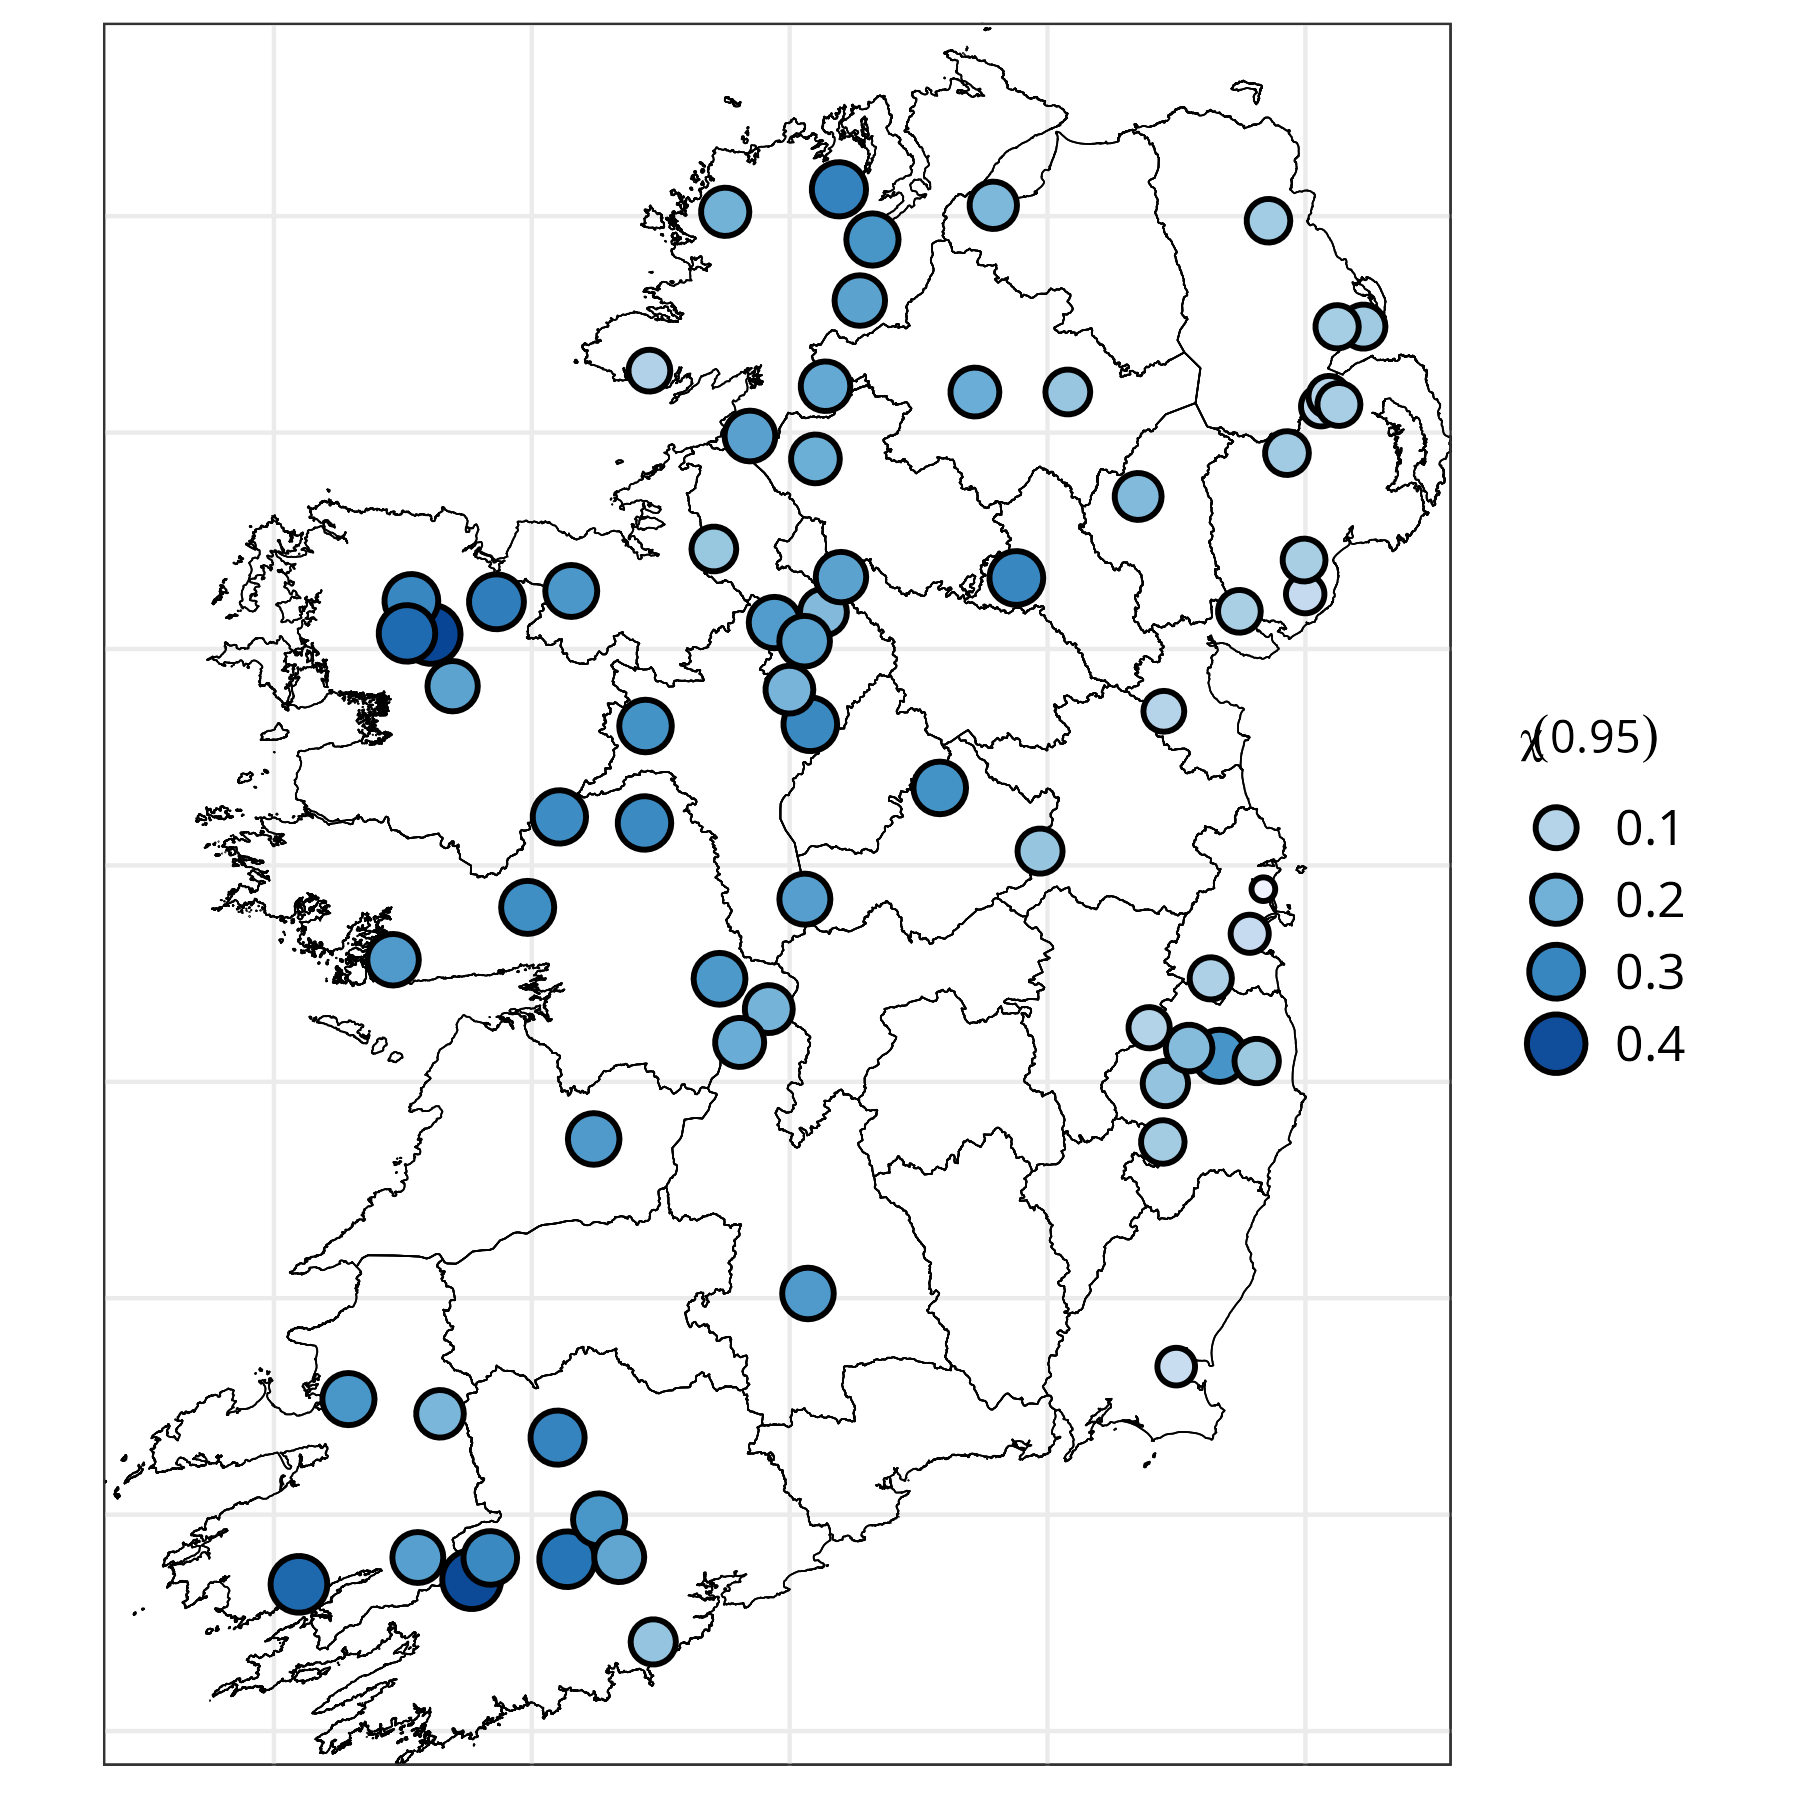
\includegraphics[width=7cm]{plots/chi_map_ire.png}
  \end{minipage}
\end{frame}


\begin{frame}{Procedure}
  \begin{itemize}
    \item Only use ECDF for marginal estimation, as spatial GPD modelling is difficult and not the focus of this analysis. 
    \item Fit the CE model to data, use clustering algorithm to cluster locations for rain $\mid$ wind speed, wind speed $\mid$ rain, and combining the $JS^{G_{\alpha}}$ dissimilarity measurements for both. 
    \item Refit CE to see if interpretation is any easier. 
  \end{itemize}
\end{frame}

\begin{frame}{$\alpha, \beta$ pre-clustering}
  \center
  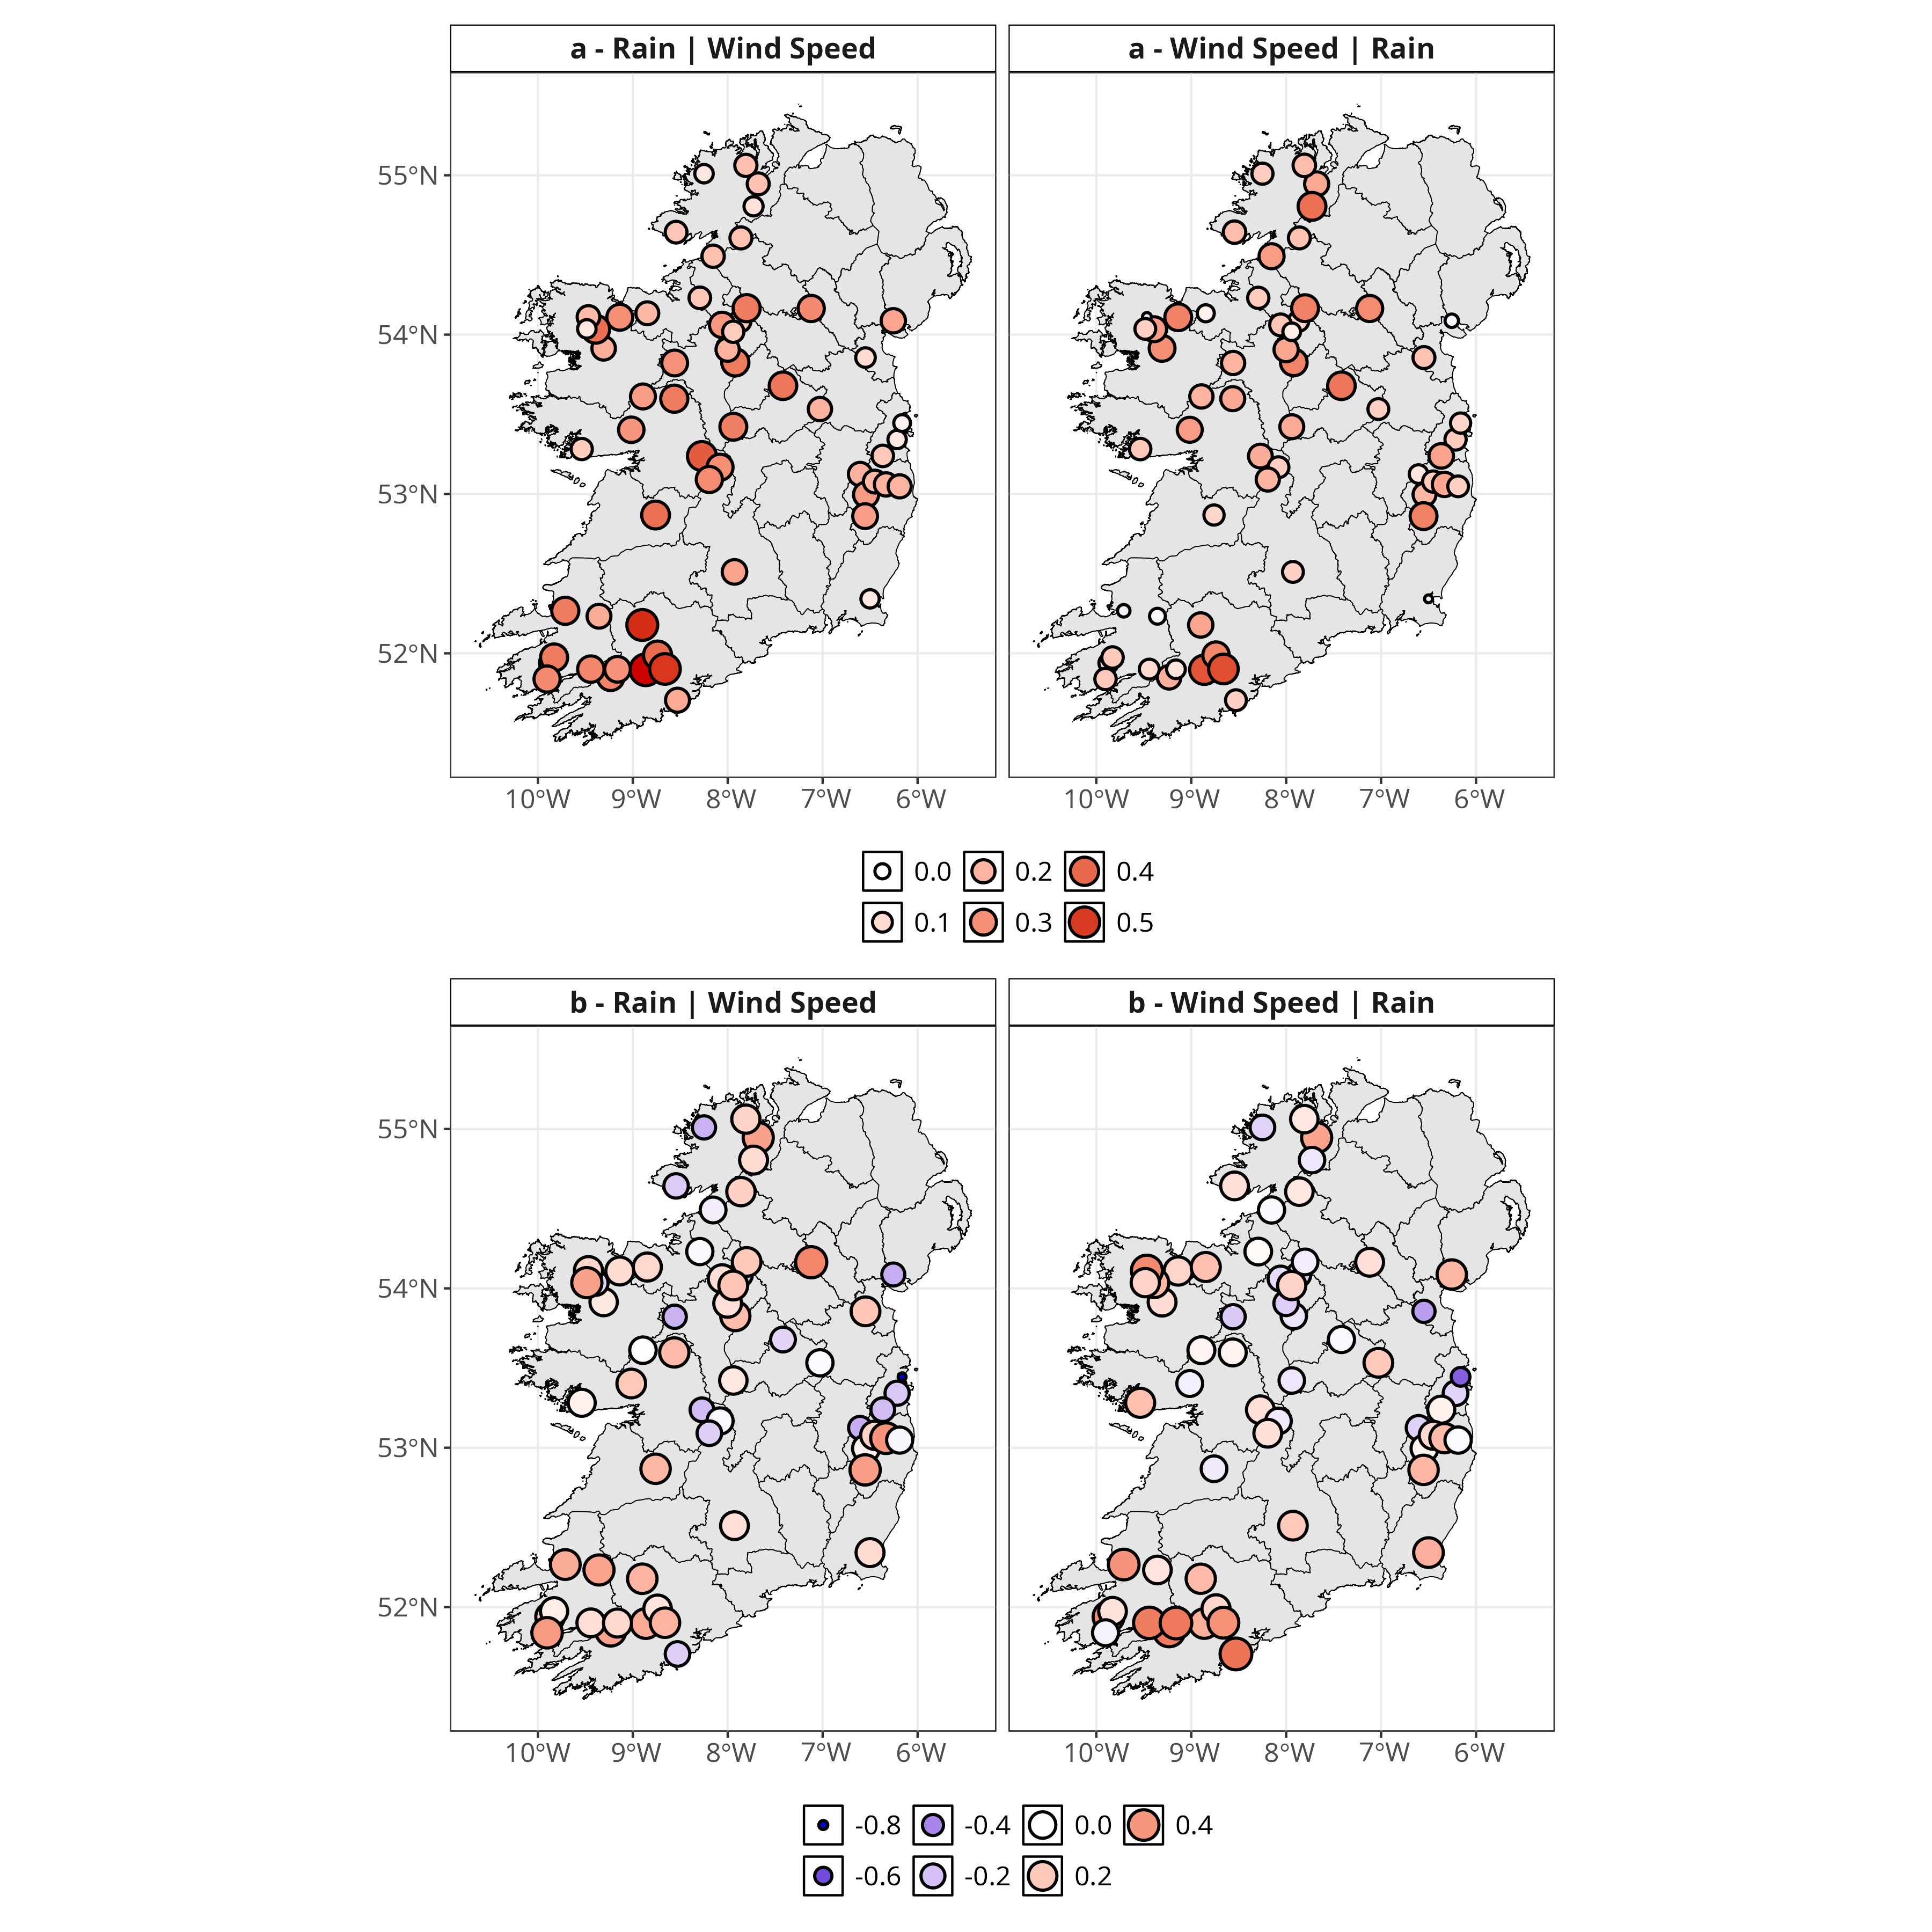
\includegraphics[width=0.78\textwidth]{plots/ire_ce.png} 
\end{frame}

% Maps of clustering
\begin{frame}{Clustering Result}
  \todo{Make county borders less bold}
  \center
  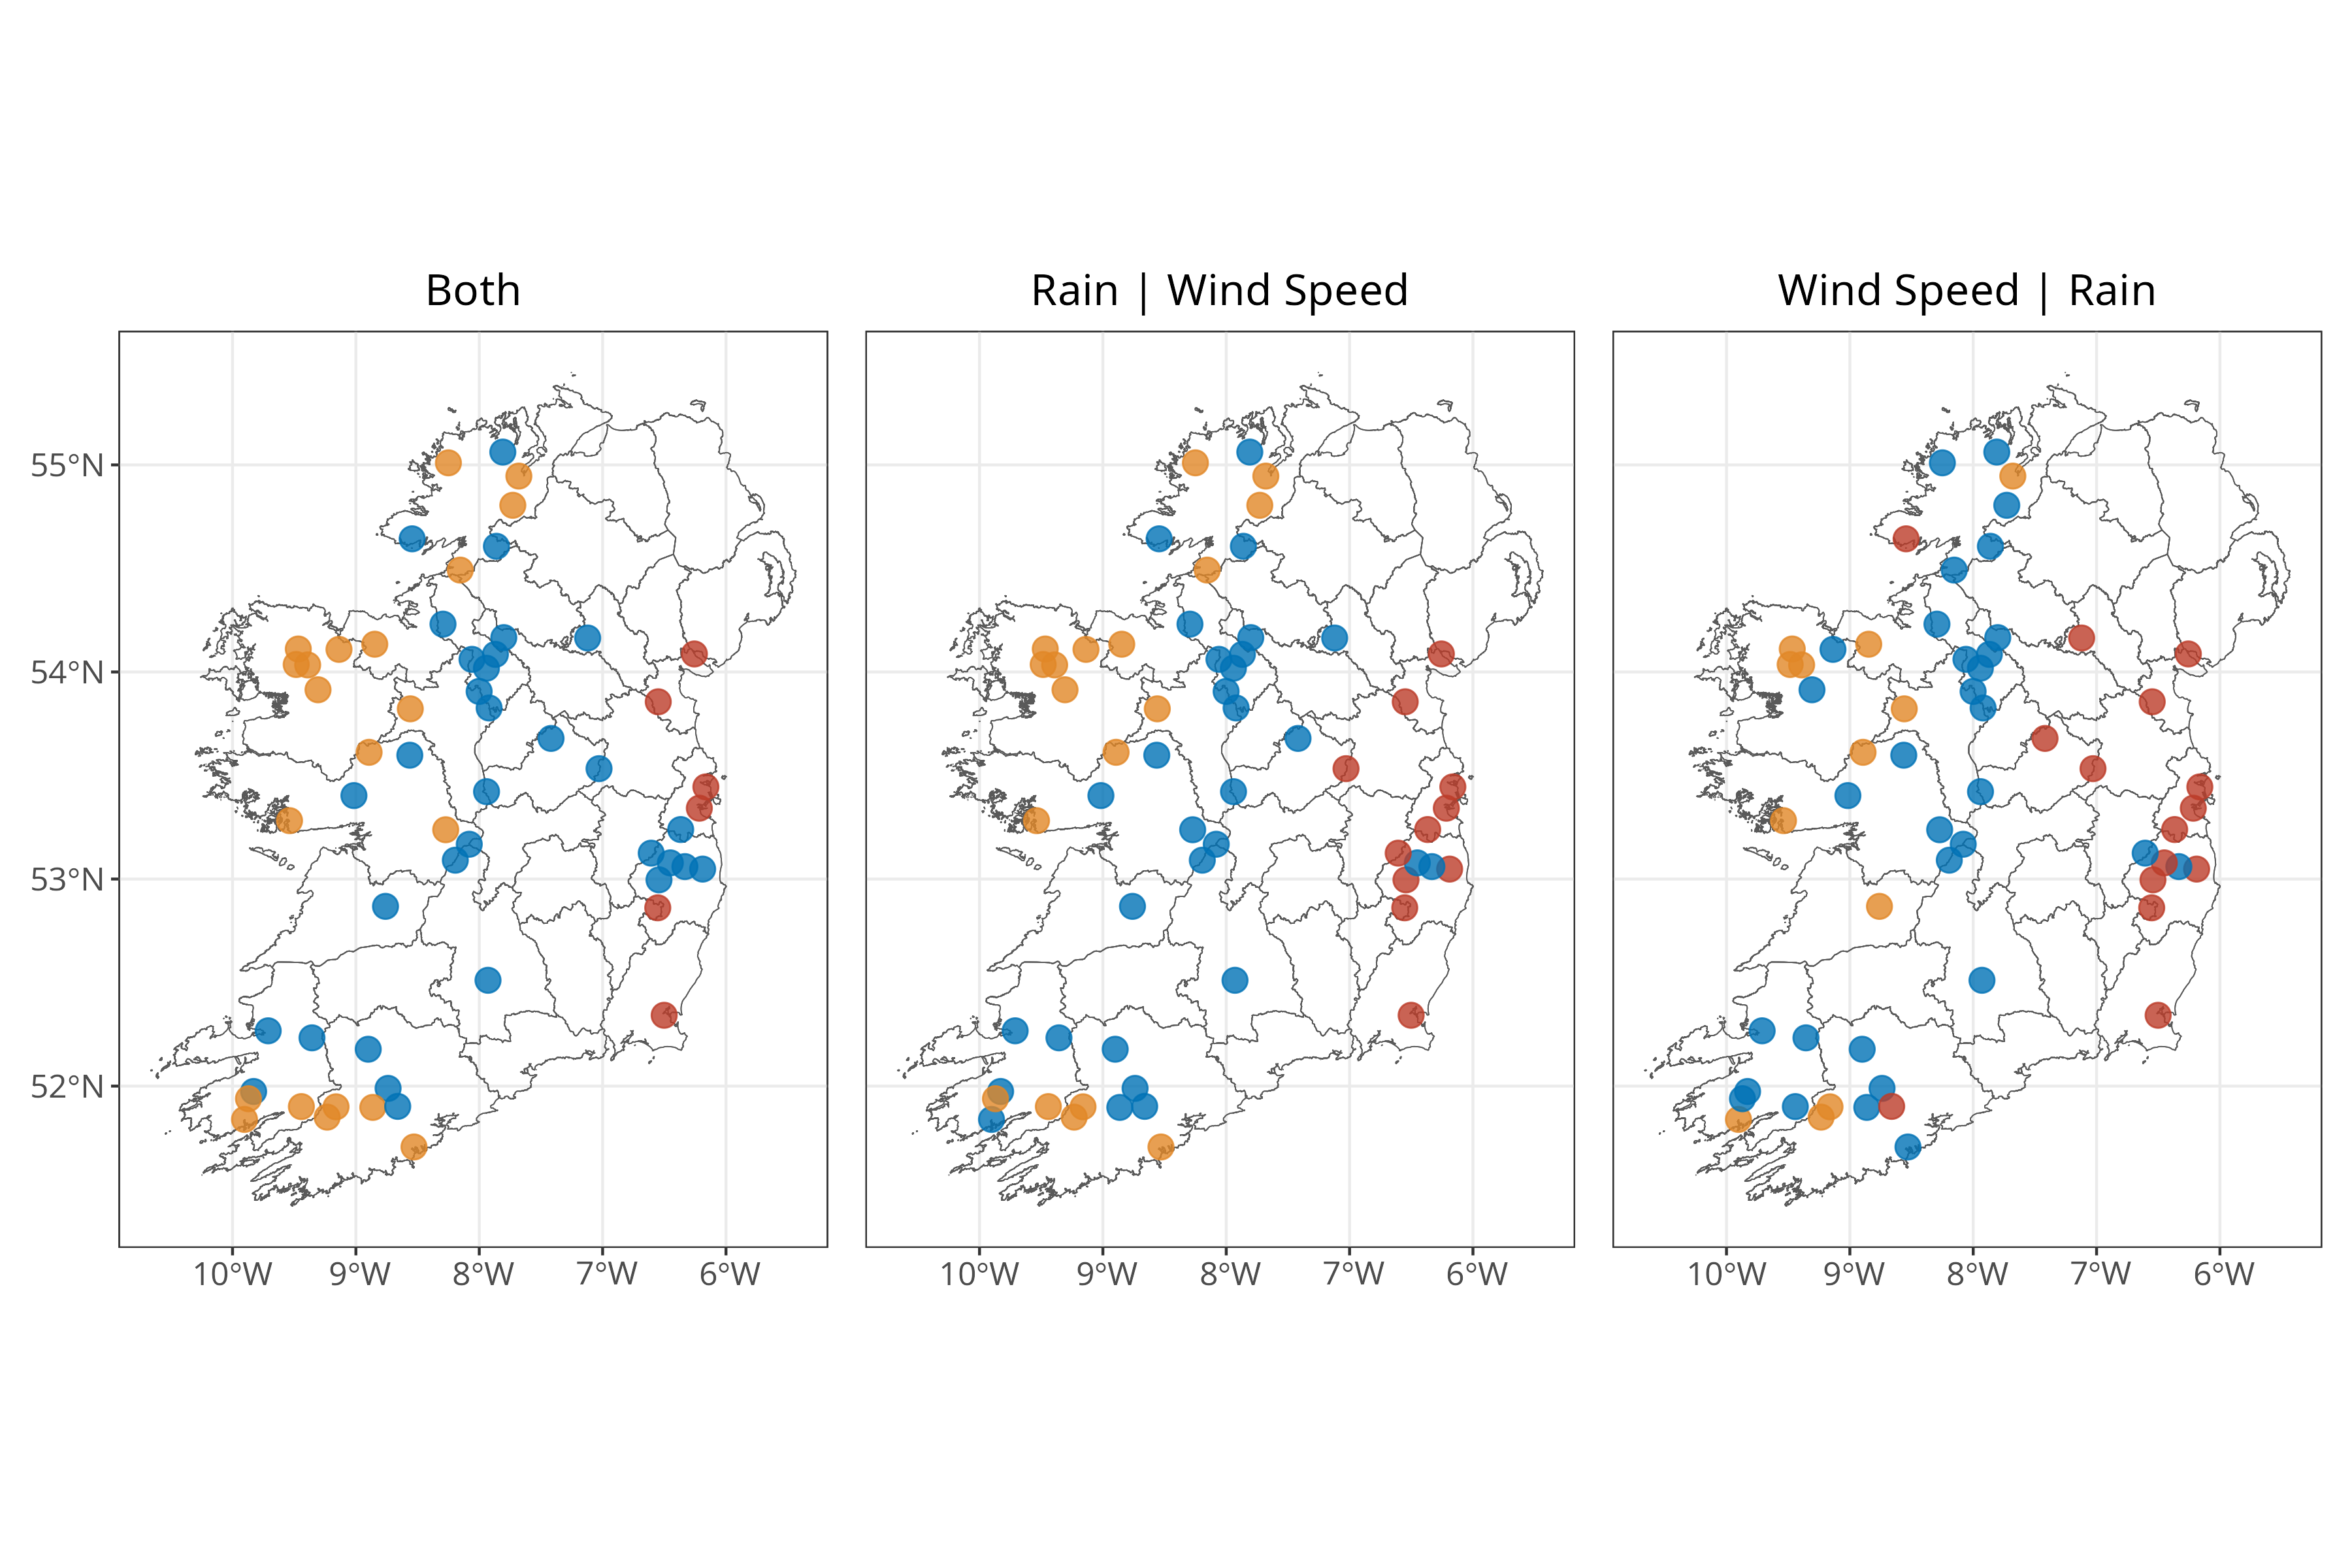
\includegraphics[width=1\textwidth]{plots/cluster_dqu_sep.pdf} 
\end{frame}

% plot of alpha, beta estimates after refitting, much more interpretable
\begin{frame}{Refitting CE model}
  % TODO: Include plots of alpha, beta estimates for each cluster, much more interpretable now!
  % 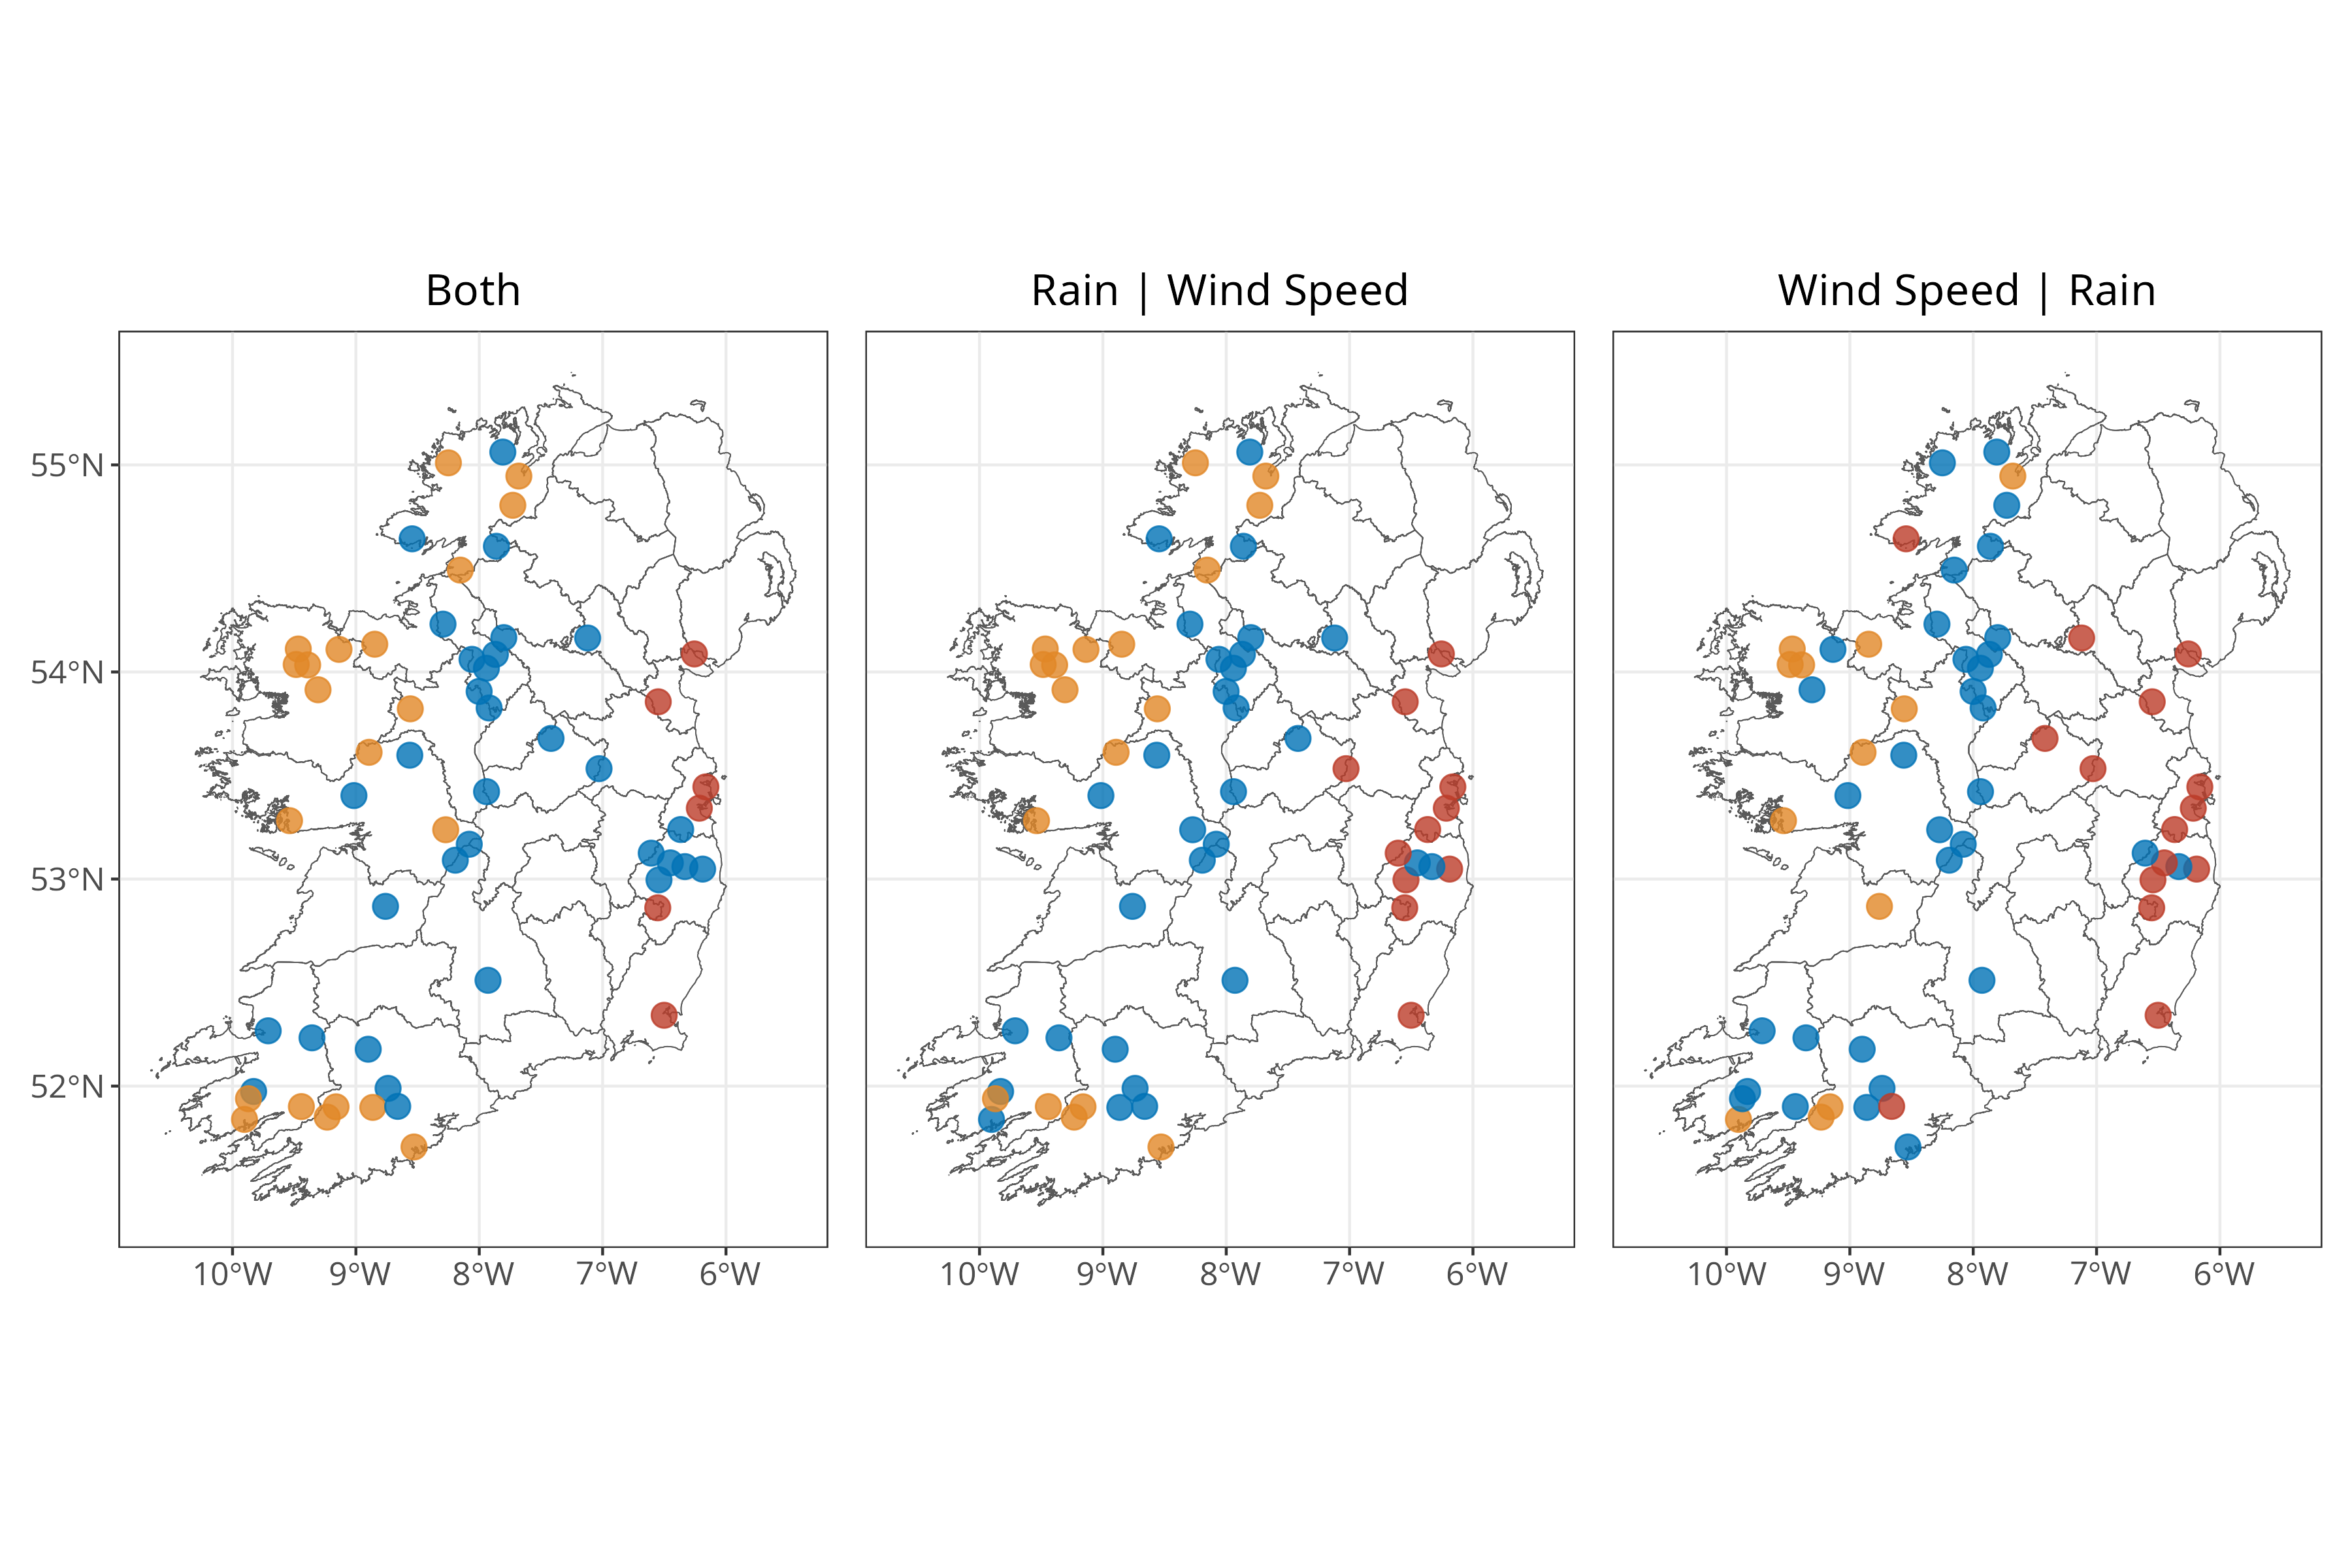
\includegraphics[width=1\textwidth]{plots/cluster_dqu_sep.pdf} 
  \center
  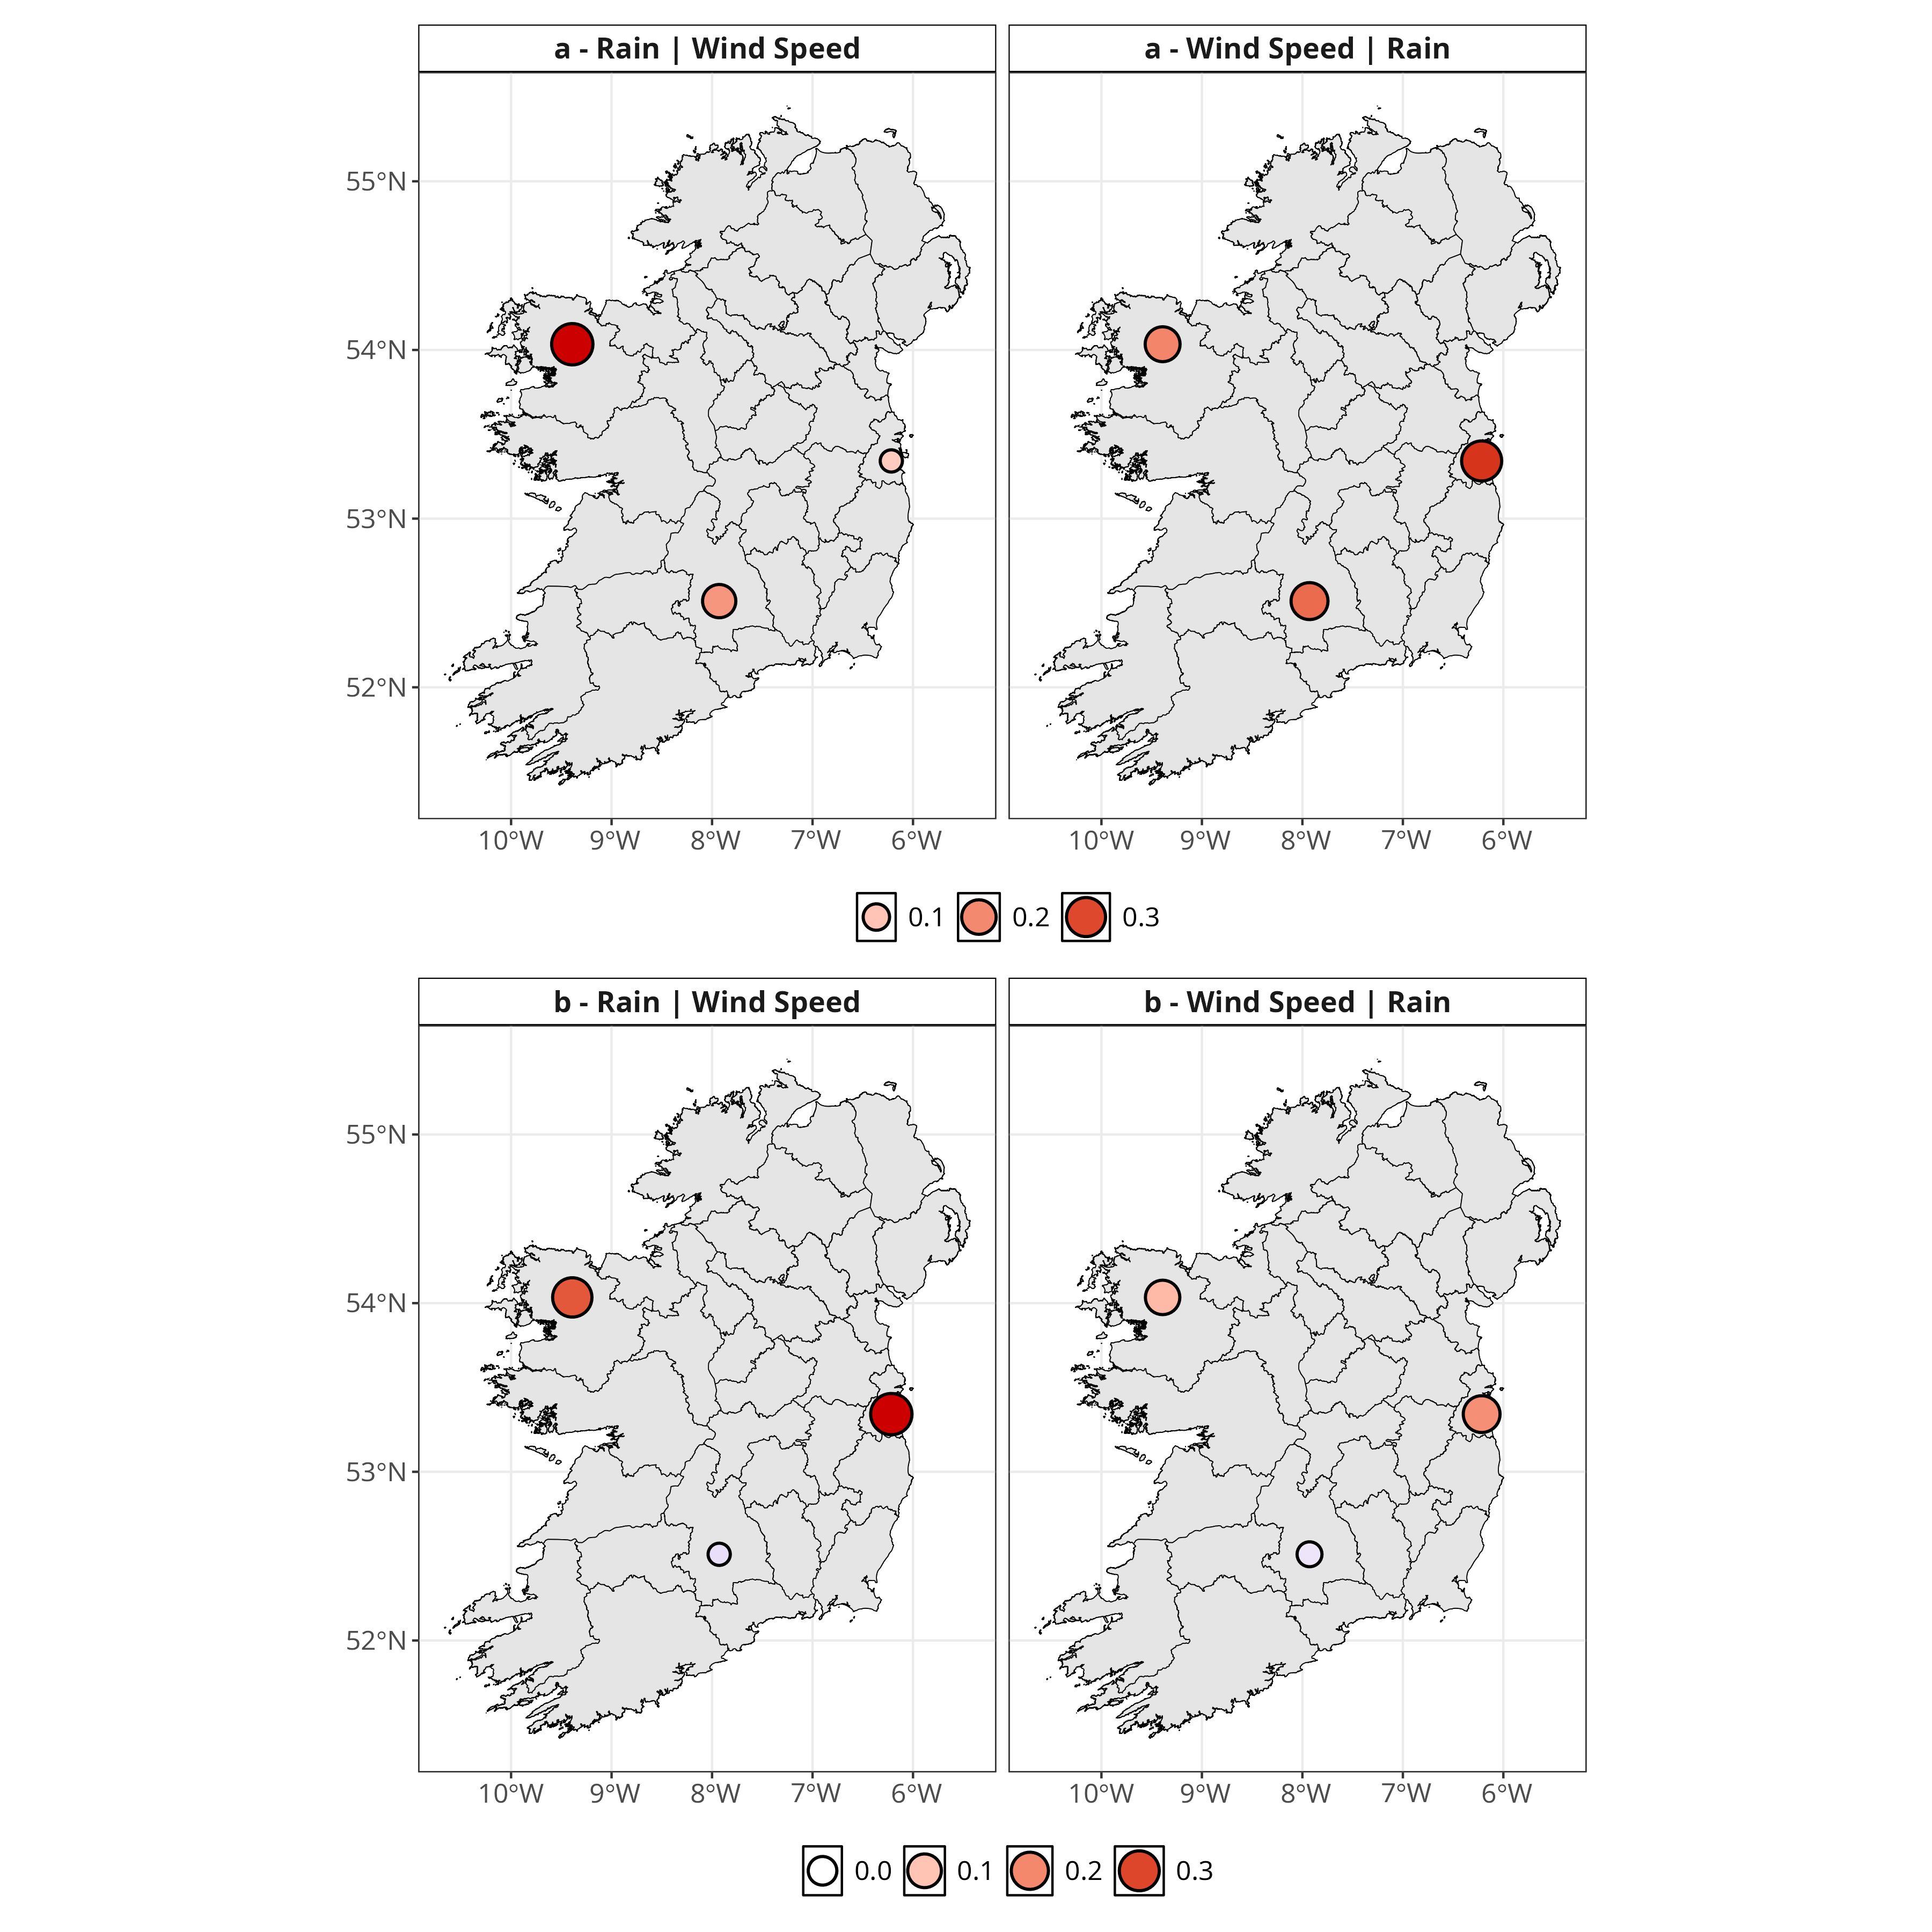
\includegraphics[width=0.78\textwidth]{plots/ab_map_post_clust.png}
\end{frame}

\begin{frame}{Refitting CE model}
  % TODO: Include plots of alpha, beta estimates for each cluster, much more interpretable now!
  % 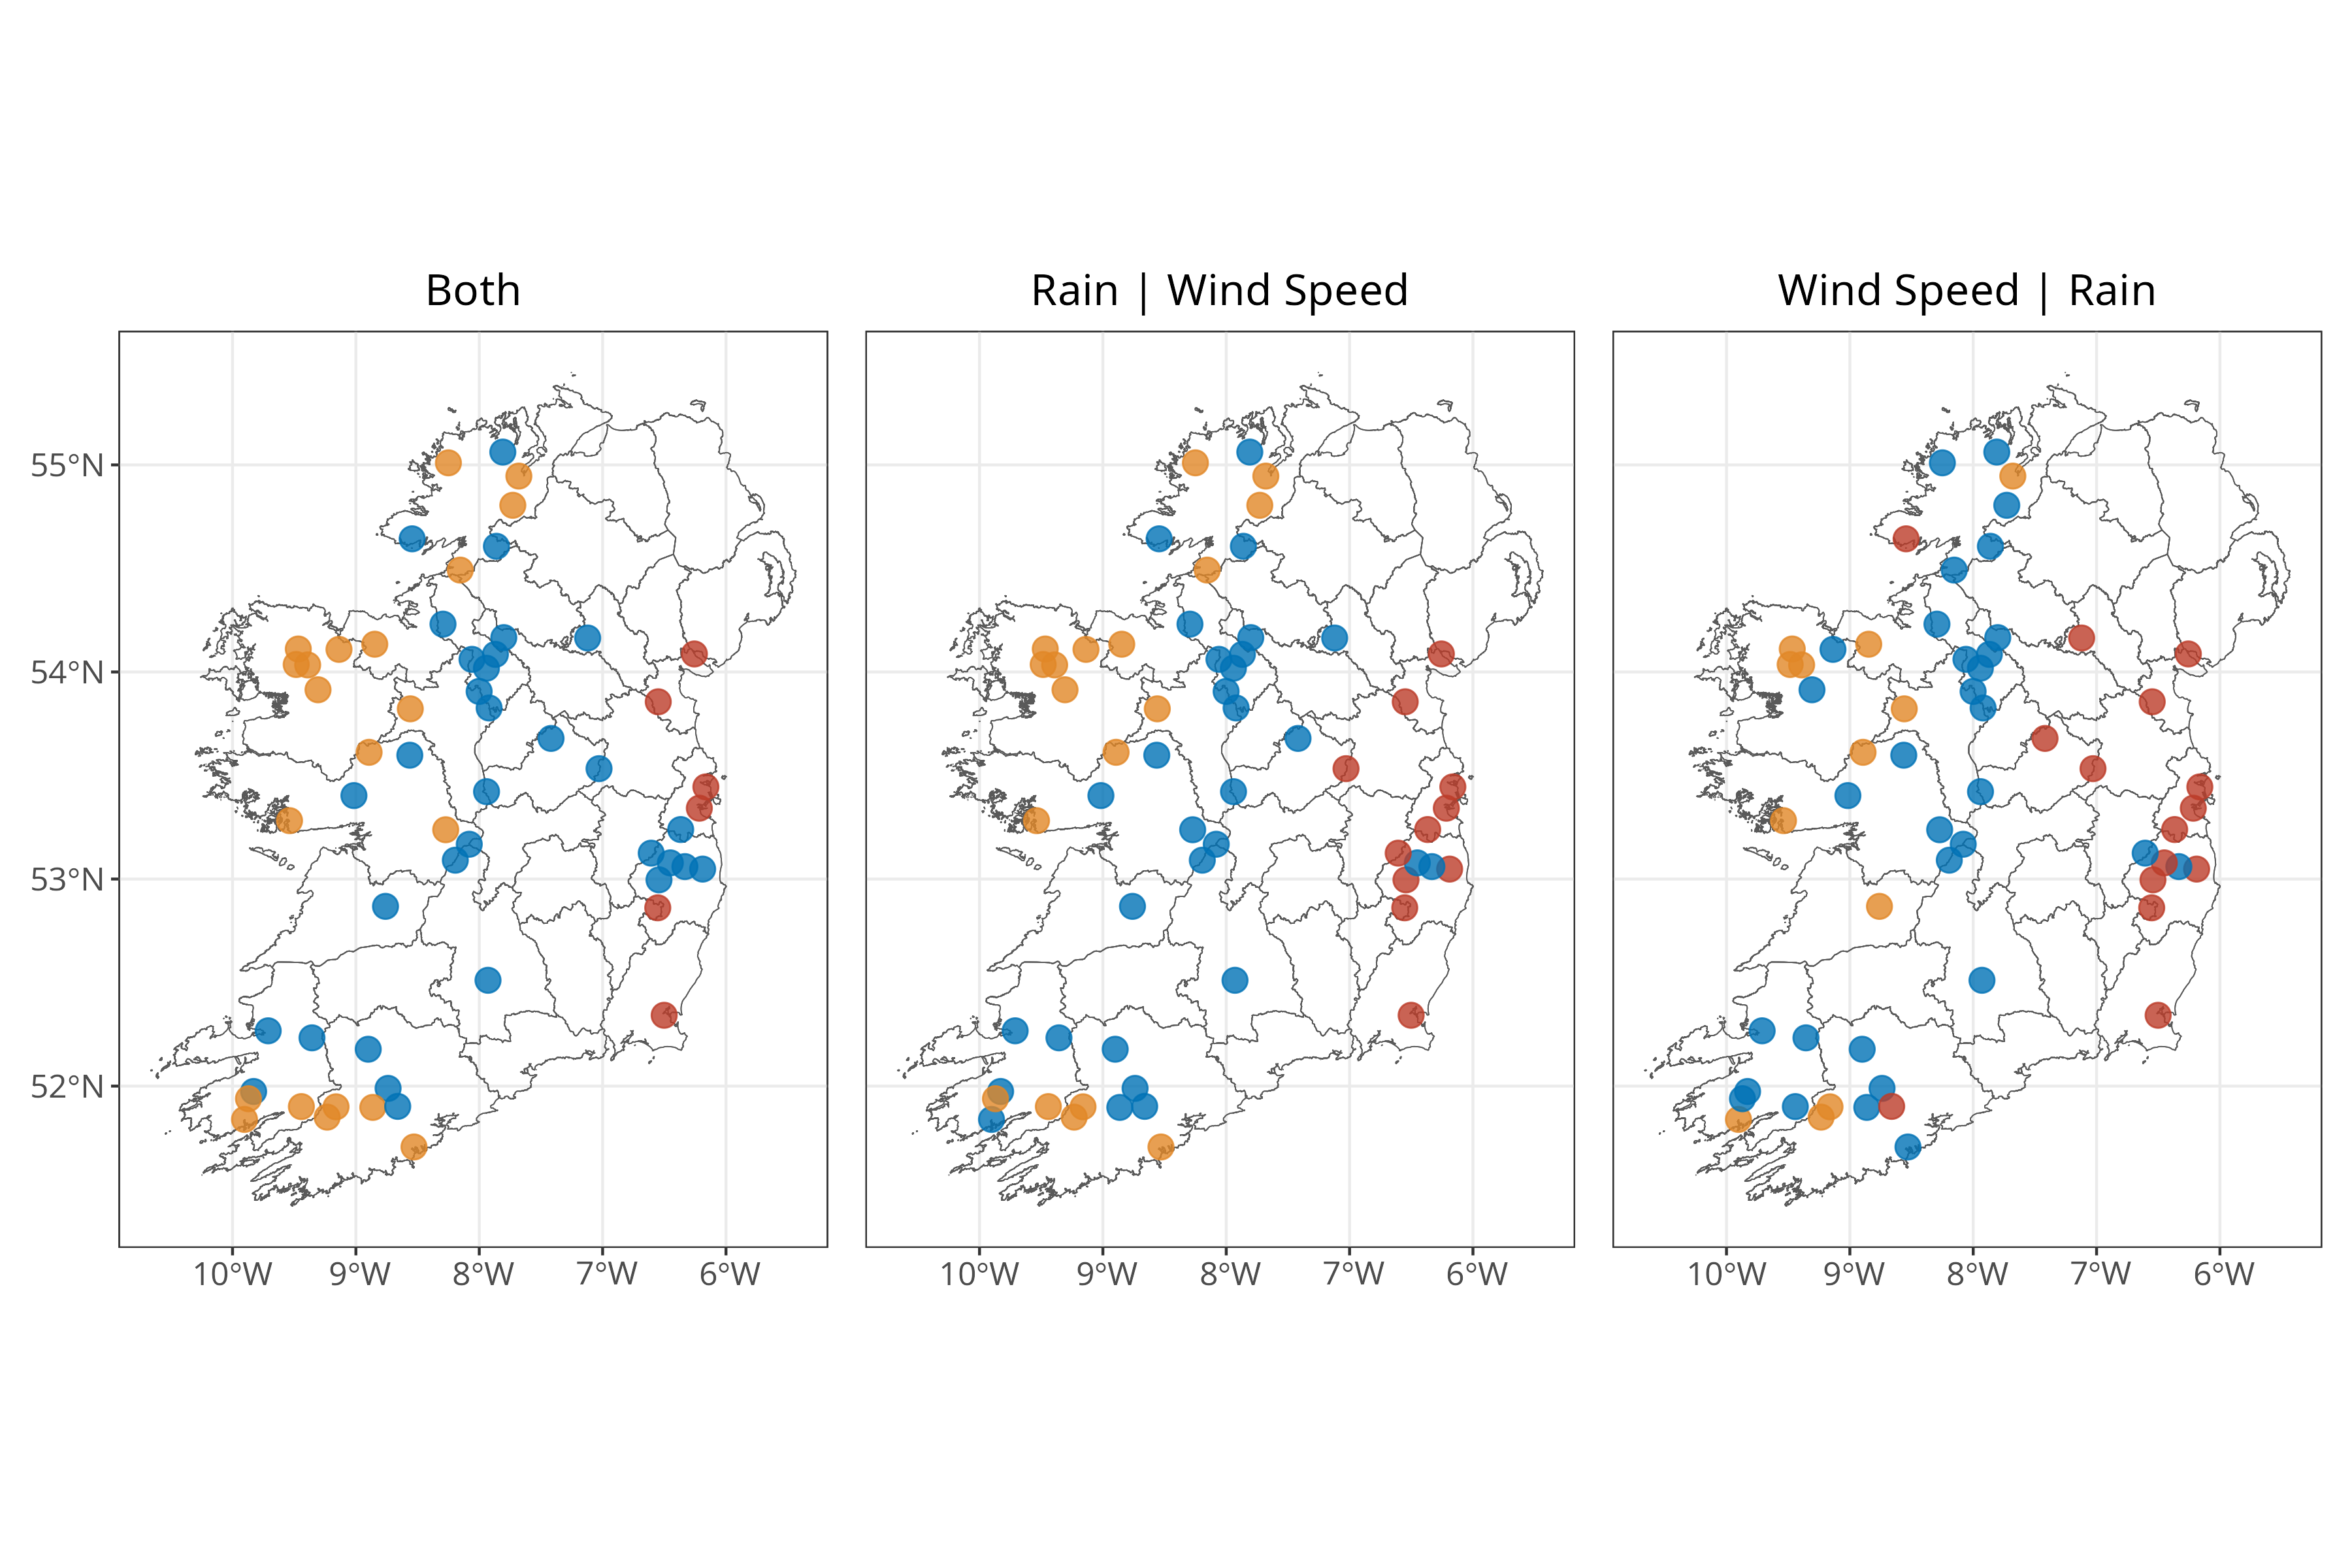
\includegraphics[width=1\textwidth]{plots/cluster_dqu_sep.pdf} 
  \center
  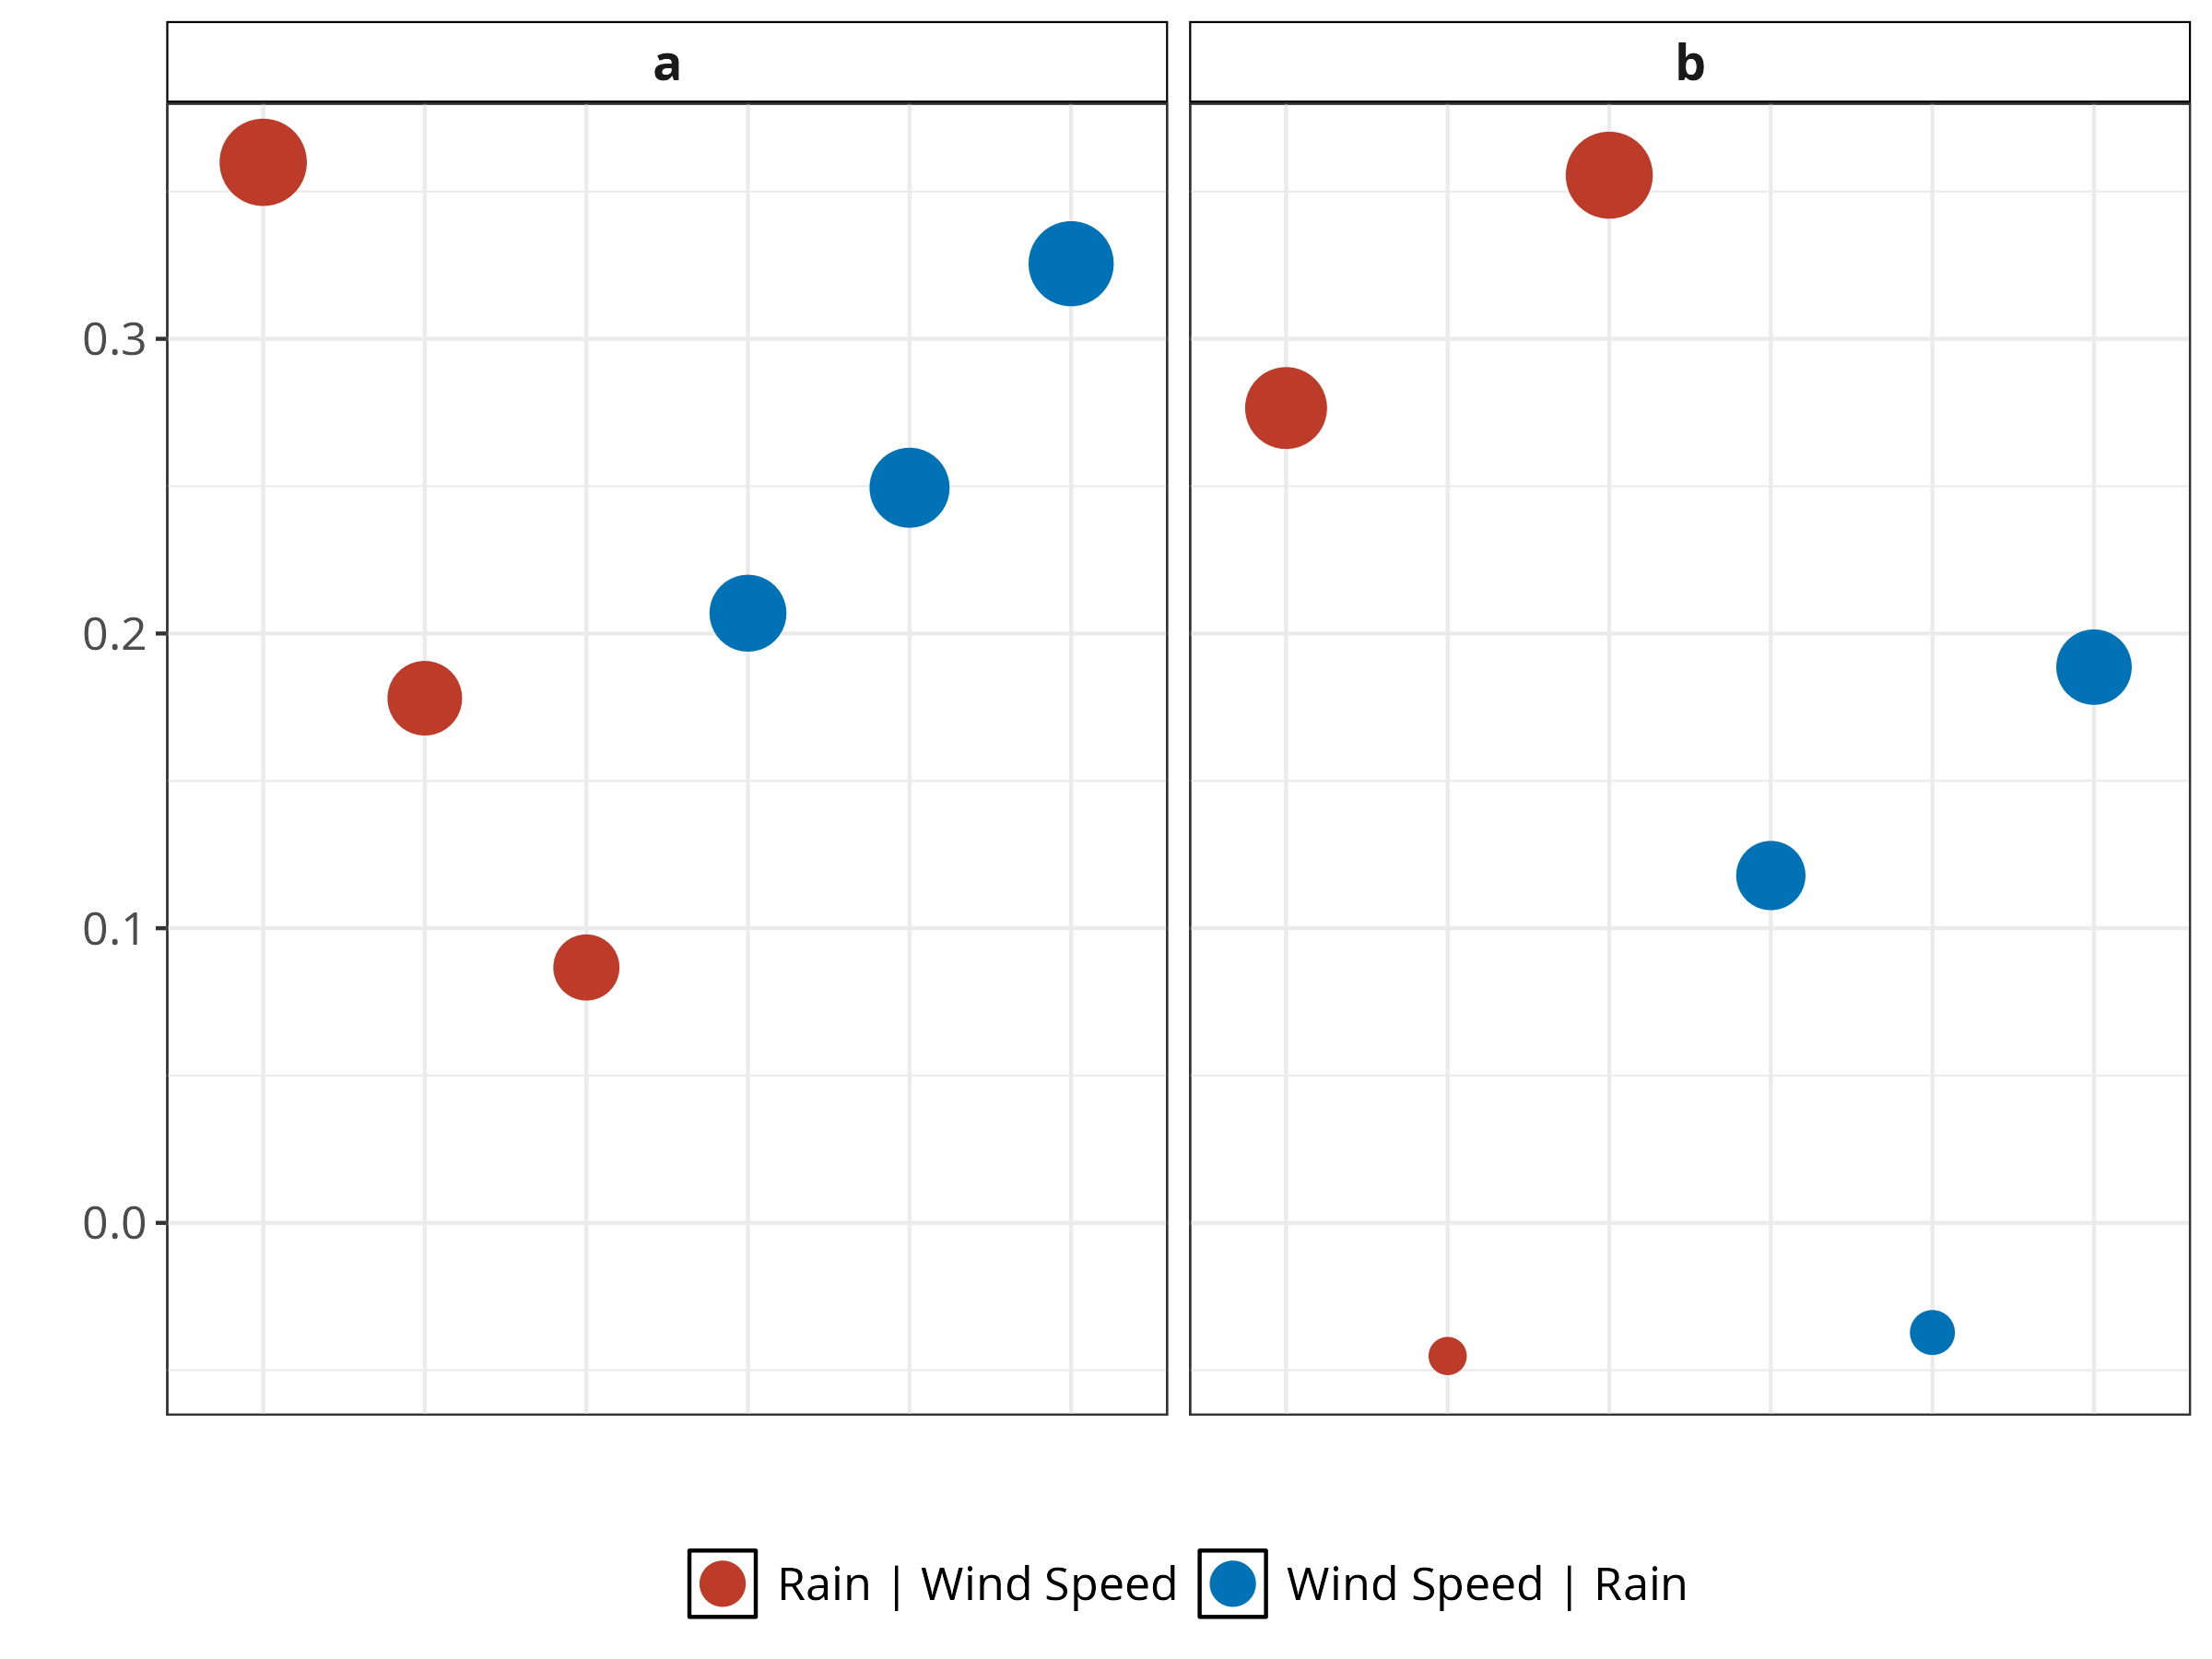
\includegraphics[width=1\textwidth]{plots/ab_post_clust.png}
\end{frame}



\section{Conclusions}

\begin{frame}{Conclusions}
\todo{Needs work!}
Limitations:
\begin{itemize}
  \item Clustering performance limited by original marginal and dependence fits, which are still to scarce data.
  \item Some $\beta$ estimates shown to be strange for Ireland.
\end{itemize}

Conclusions \& future work:
\begin{itemize}
  \item We provide a principled and effective clustering framework for CE model.
  \item Shown through simulations and real data that clustering can be used to improve interpretability of CE model.
  \item Mainly used for improved interpretability, would like to see if parameter estimation better post-clustering.
  \item Compare clustering results for Ireland to Vignotto. 
  \item Want to apply clustering to more interesting multivariate data, such as Brazil landslide data and air pollution extremes in US cities. 
\end{itemize}
\end{frame}

% TODO: Add references!
\begin{frame}\frametitle{References}
\tiny
\bibliographystyle{unsrt}
\bibliography{library.bib}
% \nocite{cocoaprod, dunn2012hadisd, faostat, hersbach2020era5, wilson2019simulation}

\end{frame}

% ===========================================================
% \frame{
% \vskip30mm
% \centerline{\Large\color{violet}\textsc{Thank you!}}
% \centerline{\Large\color{violet}\textsc{Any Questions?}}
% \vskip40mm
% }

\end{document}
